\documentclass{beamer}
\usetheme{}
\usecolortheme{dolphin}           
\useinnertheme{circles}
\setbeamertemplate{itemize items}[default]
\setbeamertemplate{enumerate items}[default]
\usepackage[T1]{fontenc}
\usepackage[utf8]{inputenc}
\usepackage{lmodern}
\usepackage{amsmath}
\usepackage{booktabs} 
\usepackage{graphicx}        
\usepackage{array}
\usepackage{color}
\makeatletter
\def\zapcolorreset{\let\reset@color\relax\ignorespaces}
\def\colorrows#1{\noalign{\aftergroup\zapcolorreset#1}\ignorespaces}
\makeatother
\graphicspath{{/home/swl/Dropbox/ucd/advanced_macro/figures/}} 
\setbeamertemplate{navigation symbols}{}

%--------------------------------------
\title{Growth accounting}
\author{School of Economics, University College Dublin}
\date{Spring 2018}
\begin{document}

%--------------------------------------
\begin{frame}
 \titlepage
\end{frame}
%--------------------------------------

%--------------------------------------
\begin{frame}
  An important early economic model on growth and living standards is Malthus' model. 
  It has two important features  
  \begin{enumerate}
    \item Long-run stagnation
    \item The idea that population growth will outpace agricultural productivity
  \end{enumerate}
\end{frame}
%--------------------------------------

%--------------------------------------
\begin{frame}
 Let's consider a simple Malthusian model where output is determined by two factors
 \begin{enumerate}
   \item Land $X$
   \item Labour $L$
 \end{enumerate}
 For simplicity we will assume that the amount of land is fixed and that the labour force will equal the total population
\end{frame}
%--------------------------------------

%--------------------------------------
\begin{frame}
  Can write the aggregate production function as
  \begin{align}
    Y=AX^{\alpha}L^{1-\alpha}
  \end{align}
  \medskip
  $Y$ is total aggregate output\\
  $A$ is technology parameter
\end{frame}
%--------------------------------------

%--------------------------------------
\begin{frame}
  Output $Y$ will increase when total population $L$ increases, but the marginal productivity will decrease as it is defined by
  \begin{align}
    \frac{\delta Y}{\delta L} &= (1-\alpha)AX^{\alpha}L^{-\alpha}\\
  &= (1-\alpha)A \left( \frac{X}{L} \right)^{\alpha} > 0
  \end{align}  
\end{frame}
%--------------------------------------

%--------------------------------------
\begin{frame}
  The marginal product is positive, meaning that an extra worker will add extra output.
  But since $L$ is in the denominator the marginal product will decrease.
  \begin{align}
    \frac{\delta^2Y}{\delta L^2} = -\alpha(1-\alpha)AX^{\alpha}L^{-\alpha-1}<0
  \end{align}
\end{frame}
%--------------------------------------

%--------------------------------------
\begin{frame}
  To measure living standard economists and policy makers often rely on output per capita as an indicator.
  We can express output per capita $y$ as
  \begin{align}
    \frac{Y}{L} &= y = \frac{AX^{\alpha}L^{1-\alpha}}{L}\\
    &= A\left ( \frac{X}{L} \right)^{\alpha} = Ax^{\alpha}
  \end{align}
  Where $x$ is land per capita.
\end{frame}
%--------------------------------------

%--------------------------------------
\begin{frame}
  An increase in population size will have two effects on living standards
  \begin{enumerate}
    \item Increase in production meaning an increase in living standards
    \item More people to share production with meaning a decrease in living standards
  \end{enumerate}
  \medskip
  According to the model the latter effect will dominate and therefore population growth will lead to a fall in living standards.  
\end{frame}
%--------------------------------------

%--------------------------------------
\begin{frame}
 More formally;
 \begin{align}
  \frac{\delta y}{\delta L} &= -\alpha AX^{\alpha}L^{-\alpha-1} <0\\
  \frac{\delta^2 y}{\delta L^2} &= \alpha(1-\alpha)AX^{\alpha}L^{-\alpha-2}>0
 \end{align}  
\end{frame}
%--------------------------------------

%--------------------------------------
\begin{frame}
 Given the dynamics between population and output growth, let's have a closer look at population dynamics. 
 We let population size $L_t$ is equal last year's population size plus the number of births $B_t$ and minus the number of deaths $D_t$ during the same year, or
  \begin{align}
   L_t = L_{t-1} + B_t(y_{t-1}) - D_t(y_{t-1})
  \end{align}
  \medskip
  Key feature here is that the number of births and deaths is a function of living standards or output per capita, lagged one year: $y_{t-1}$
  \begin{align}
    B'(y_{t-1})&>0\\
    D'(y_{t-1})&<0  
  \end{align}
  \medskip
  For simplicity the birth and death rate are assumed to be linear functions of output.
\end{frame}
%--------------------------------------

%--------------------------------------
\begin{frame} 
  \begin{figure}
    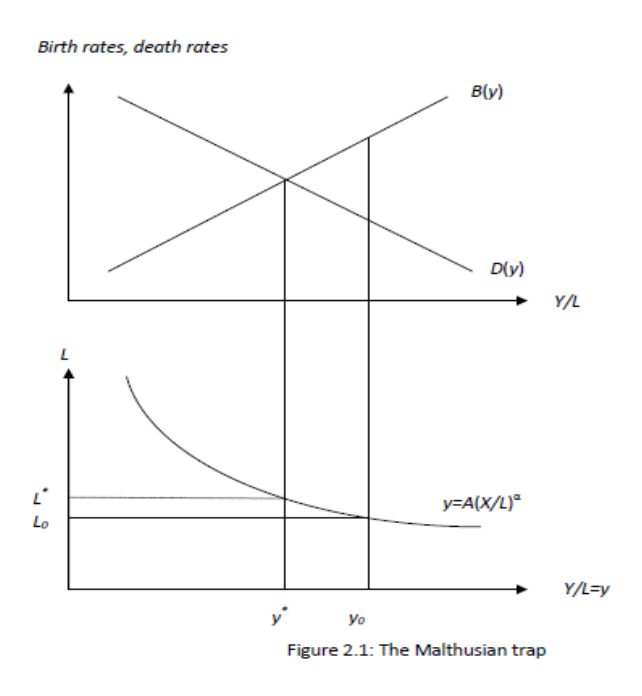
\includegraphics[scale=.7]{malthusian_trap.eps}
  \end{figure}
\end{frame}
%--------------------------------------

%--------------------------------------
\begin{frame}
  So when output per capita increases, the food supply will increase which allows families to expand and reduce mortality due to better nourishment. 
  Output per capita will tend to converge towards an equilibrium indicated by $y^*$, at which point the population ceases to grow.
  \begin{itemize}
    \item This is known as the subsistence level
  \end{itemize}
  \begin{align}
  L_t-L{t-1} = B_t(y^*)-D_t(y^*)=0
  \end{align}
\end{frame}
%--------------------------------------

%--------------------------------------
\begin{frame}
  Consider the case where we start at a relatively high output level, $y^0$.
  Given the relatively high output per capita there will be (relatively)
  \begin{itemize}
    \item Few deaths
    \item Many births
  \end{itemize}
  \medskip
  This will increase the population, decreasing living standards shifting the equilibrium to the left. 
  \begin{itemize}
    \item One can imagine a scenario starting at the left of the equilibrium where many people die and few children are born
    \item In this case the shrinking population will increase output per capita
  \end{itemize}
\end{frame}
%--------------------------------------

%--------------------------------------
\begin{frame}
  \begin{figure}
    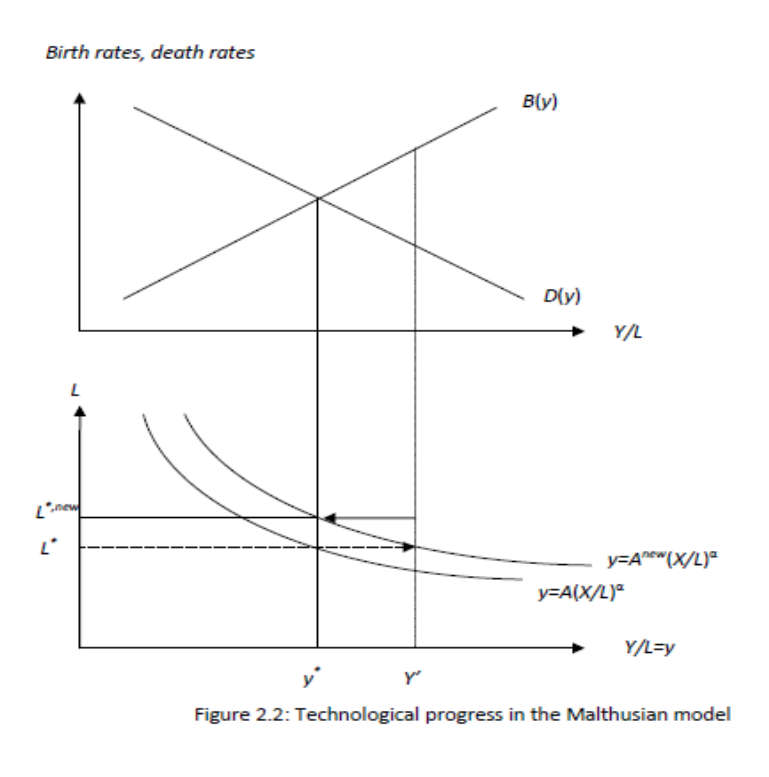
\includegraphics[scale=.7]{tech_progress.eps}
  \end{figure}
\end{frame}
%--------------------------------------

%--------------------------------------
\begin{frame}
  Consider a positive technology shock increasing productivity. 
  \begin{itemize}
    \item Productivity increase will shift equilibrium punt outward on $y$-curve: temporary increase in output per capita
    \item This will increase birth rate and decrease death rate
    \item Population will increase reducing the living standards
  \end{itemize}
  \medskip
  As such, the only lasting thing of a technology shock is a larger population.
\end{frame}
%--------------------------------------

%--------------------------------------
\begin{frame}
History has shown however that there are a number of factors that can contribute to a break with the Malthusian trap. 
\begin{enumerate}
  \item Fall in birth rate ending link with income per capita
  \item Increase in education level
  \item Increase in growth of technological knowledge
  \item Increase in output per capita far beyond subsistence level
\end{enumerate}
\end{frame}
%--------------------------------------

%--------------------------------------
\begin{frame}
 Let's have a look at the Cobb-Douglas model  
\begin{align}
  Y_t=A_tK^{\alpha}_tL^{\beta}_t
\end{align}
  \medskip
  Assume that output is determined by an aggregate production function technology depending on the total amount of labour ($L$) and capital ($K$). 
\end{frame}
%--------------------------------------

%--------------------------------------
\begin{frame}
  In the Cobb-Douglas model $A_t$ accounts for technology, a measure for productive efficiency
\begin{itemize}
  \item Increase in $A_t$ results in higher output without having to raise inputs
  \item Fluctuates for various reasons, e.g. new technology, government regulation, better management
\end{itemize} 
\medskip
Since $A_t$ increases productiveness of other factors, it is also known as Total Factor Productivity (TFP)
\end{frame}
%--------------------------------------

%--------------------------------------
\begin{frame}
  We are often interested in the output per worker or productivity.
  Output per worker is given by
  \begin{align}
    \frac{Y_t}{L_t}=A_tK^{\alpha}L^{\beta-1}_t=A_t \left(\frac{K_t}{L_t} \right)^{\alpha}L_t^{\alpha+\beta-1}
  \end{align}
  Increases in output per worker is productivity growth.
\end{frame}
%--------------------------------------

%--------------------------------------
\begin{frame}
  \begin{figure}
    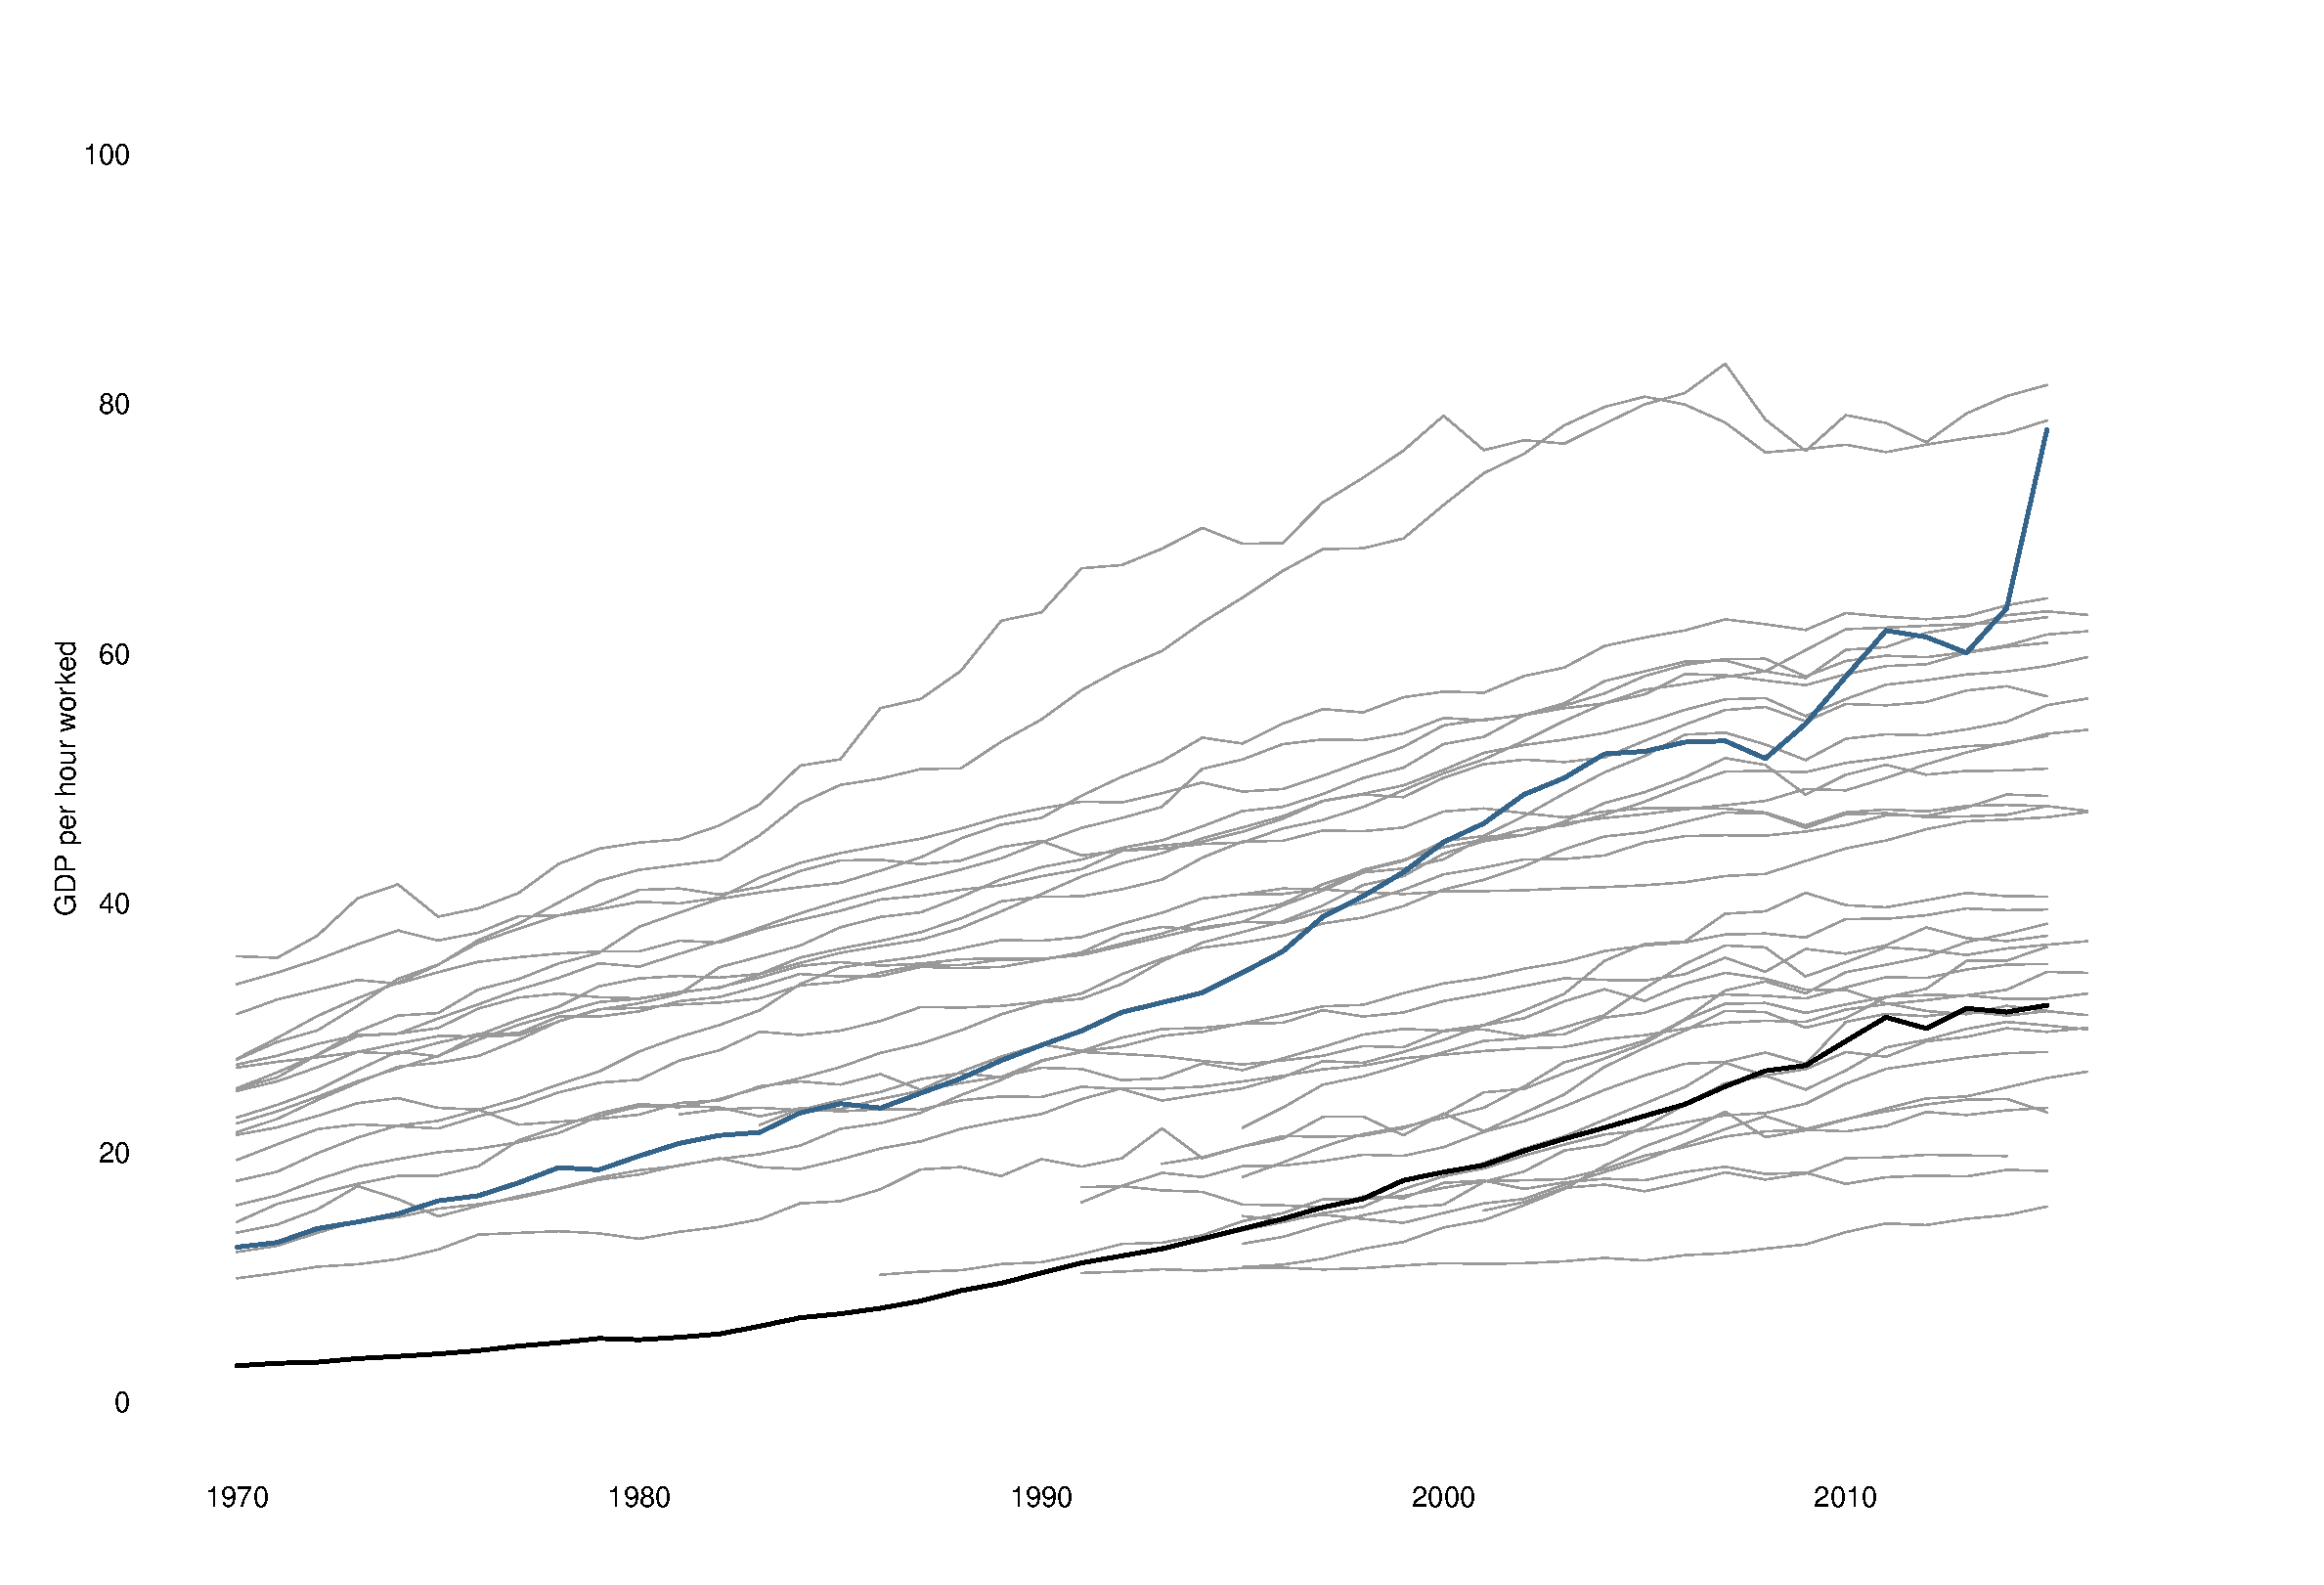
\includegraphics[scale=.3]{productivity.eps}
  \end{figure}
\end{frame}
%--------------------------------------

%--------------------------------------
\begin{frame}
 There are three way to increase productivity
This function shows that there are three potential ways to increase productivity
\begin{enumerate}
  \item Increase in labour force  
  \item Technological progress; Improving the efficiency of the economy
  \item Capital deepening: Increasing the amount of capital per worker  
\end{enumerate}
\end{frame}
%--------------------------------------

%--------------------------------------
\begin{frame}
 Concerning growth of the labour force; increasing the number of workers will only add to growth if
 \begin{align}
   \alpha+\beta>1
 \end{align}
 \medskip
 i.e. under increasing returns to scale, whereas most growth theories assume constant returns to scale (CRS).
 \begin{align}
   \alpha+\beta &= 1\\
   \frac{Y_t}{L_t} &= A_t \left(\frac{K_t}{L_t}\right)^{\alpha}
 \end{align}
\end{frame}



%--------------------------------------
\begin{frame}
  Let's examine what determines growth under the CRS assumptions.
  Given   
  \begin{align}
   \alpha+\beta &= 1
  \end{align}
  We get
  \begin{align}
    Y_t=A_tK^{\alpha}_tL^{1-\alpha}_t
  \end{align}
  \medskip
  Time is assumed to be continuous
  \begin{itemize}
    \item $t$ evolves smoothly instead of taking integer values like $t=1,t=2,...$.
  \end{itemize}
  \medskip
  The growth rate of $Y_t$ can be denoted by $G^Y_t$ and defined as
  \begin{align}
    G^Y_t=\frac{1}{Y_t}\frac{dY_t}{dt}
  \end{align}
  i.e growth equals the change in output divided by output level.
\end{frame}
%--------------------------------------

%--------------------------------------
\begin{frame}
  Can differentiate production function with respect to time; expressing it as a function of $G^Y_t$ 
  \begin{itemize}
    \item Can define the growth rates of labour, capital, and technology. 
  \end{itemize}
  \begin{align}
    \frac{dK_t^{\alpha}}{dt} &= \frac{dK_t^{\alpha}}{dK_t}\frac{dK_t}{dt} =\alpha K_t^{\alpha-1}\frac{dK_t}{dt}\\
    \frac{dL_t^{1-\alpha}}{dt} &= \frac{dL_t^{1-\alpha}}{dL_t}\frac{dL_t}{dt} = (1-\alpha)L_t^{-\alpha}\frac{dL_t}{dt}
  \end{align}
\end{frame}
%--------------------------------------

%--------------------------------------
\begin{frame}
 For the next step we need to use the product rule, which implies
\begin{align}
  \frac{dABC}{dx}=BC\frac{dA}{dx}+AC\frac{dB}{dx}+AB\frac{dC}{dx}
\end{align}
\end{frame}
%--------------------------------------

%--------------------------------------
\begin{frame}
 Also using the chain rule, for the whole production function we can calculate the terms involving the impact of changes in capital and labour inputs as
  \begin{align}
    \frac{dY_t}{dt} &= \frac{dA_tK_t^{\alpha}L_t^{1-\alpha}}{dt}\\
    &= K_t^{\alpha}L_t^{1-\alpha}\frac{dA_t}{dt} + A_tL_t^{1-\alpha}\frac{dK_t^{\alpha}}{dt} + A_tK_t^{\alpha}\frac{dL_t^{1-\alpha}}{dt}\\
    &= K_t^{\alpha}L_t^{1-\alpha}\frac{dA_t}{dt} + \alpha A_tK_t^{\alpha-1}L_1^{1-\alpha} \frac{dK_t}{dt}  + (1-\alpha)A_tK_t^{\alpha}L_t^{-\alpha}\frac{dLt}{dt}
  \end{align}
\end{frame}
%--------------------------------------

%--------------------------------------
\begin{frame}
  We can now calculate the growth rate of output by dividing boths sides by $Y_t$.   
  \begin{align}
    \frac{1}{Y_t}\frac{dY_t}{dt} & = \frac{K_t^{\alpha}L_t^{1-\alpha}}{A_tK_t^{\alpha}L_t^{1-\alpha}} \frac{dA_t}{dt} + \\& \alpha \frac{A_tK_t^{\alpha-1}L_1^{1-\alpha}}{A_tK_t^{\alpha}L_t^{1-\alpha}} \frac{dK_t}{dt} + (1-\alpha) \frac{A_tK_t^{\alpha}L_t^{-\alpha}}{A_tK_t^{\alpha}L_t^{1-\alpha}} \frac{dLt}{dt}\\
    \frac{1}{Y_t}\frac{dY_t}{dt} & = \frac{1}{A_t}\frac{dA_t}{dt} + \alpha \frac{1}{Kt}\frac{dK_t}{dt} + (1-\alpha) \frac{1}{L_t}\frac{dL_t}{dt}\\ 
    G_t ^Y &=G_t^A +\alpha G_t^K + (1-\alpha)G_t^L
\end{align}
  \medskip
  NB- This is the same as dividing by $A_tK_t^{\alpha}L_t^{1-\alpha}$
\end{frame}
%--------------------------------------

%--------------------------------------
\begin{frame}
  This shows that output growth equals technology growth plus a weighted average of the growth rates of capital and labour
  \begin{itemize}
    \item With the weight determined by $\alpha$
  \end{itemize}
  \medskip
  This is the key equation in growth accounting studies. 
\end{frame}
%--------------------------------------

%--------------------------------------
\begin{frame}
  Growth accounting studies provide estimates of how much GDP growth over a certain time span is determined by 
  \begin{enumerate}
    \item Growth in the number of workers
    \item Growth in capital stock
    \item Improvement in Total Factor Productivity
  \end{enumerate}
\end{frame}
%--------------------------------------

%--------------------------------------
\begin{frame}
Calculating the growth equation
\begin{align}
  G_t ^Y &=G_t^A +\alpha G_t^K + (1-\alpha)G_t^L
\end{align}
\medskip
requires
\begin{itemize}
  \item A measure for output i.e. GDP
  \item Number of workers
  \item Capital stock estimate 
  \item Value for Total Factor Productivity
\end{itemize}
\end{frame}
%--------------------------------------

%--------------------------------------
\begin{frame}
One empirical issue is that the value for TFP ($A_t$) can't be directly observed. 
However, if we know the value of parameter $\alpha$ we can get an estimate for growth. 
\begin{align}
  G_t ^A &=G_t^Y -\alpha G_t^K - (1-\alpha)G_t^L
\end{align}
\end{frame}
%--------------------------------------

%--------------------------------------
\begin{frame}
  Solow (1957) pointed out that an $\alpha$ estimate could be obtained by looking at the shares of GDP paid to workers and to capital. 
  To illustrate, consider a perfectly competitive firm that is seeking to maximise profits and the firm
  \begin{itemize}
    \item Sells product at price $P_t$
    \item Pays wages $W_t$
    \item Rents its capital at a rate of $R_t$
  \end{itemize}
\end{frame}
%--------------------------------------

%--------------------------------------
\begin{frame}
  The firm's profits are given by
  \begin{align}
    \Pi_t &= P_tY_t - R_tK_t -W_tL_t\\
    &= P_tA_tK_t^{\alpha}L_t^{1-\alpha}-R_tK_t - W_tL_t  
  \end{align}
\end{frame}
%--------------------------------------

%--------------------------------------
\begin{frame}
  The firm only needs to decide how much labour and capital to use
  It will therefore maximise profits by differentiating the function with respect to capital and labour and the the derivatives equal to zero which provides two conditions
\begin{align}
  \frac{\delta \Pi_t}{\delta K_t} &= \alpha P_tA_tK_t^{\alpha-1}L_t^{1-\alpha} -R_t = \alpha \frac{P_tY_t}{K_t} - R_t = 0\\
  \frac{\delta \Pi_t}{\delta L_t} &= (1-\alpha) P_tA_tK_t^{\alpha}L_t^{-\alpha} - W_t = (1-\alpha) \frac{P_tY_t}{L_t}- W_t = 0
\end{align}
Rearranging we get
\begin{align}
  \alpha &= \frac{R_tK_t}{P_tY_t}\\
  1-\alpha &= \frac{W_tL_t}{P_tY_t}
\end{align}
\end{frame}
%--------------------------------------

%--------------------------------------
\begin{frame}
We have that 
\begin{itemize}
  \item $P_t Y_t$ is total nominal GDP
  \item $W_t L_t$ is the total amount of income paid to wages
  \item $R_t K_T$ is the total amount of income paid to capital
\end{itemize}

$\alpha$ will be the total amount of income paid to capital relative to total income, at the aggregate level nominal GDP
\begin{itemize}
  \item $1-\alpha$ can be calculated as the fraction of income paid to workers instead of compensating capital.
\end{itemize}
\end{frame}
%--------------------------------------

%--------------------------------------
\begin{frame}
Solow found that for most countries the national income accounts show that wage income explains most of GDP, corresponding to $\alpha<0.5$
  \begin{itemize}
    \item Based on the estimates for the US economy, commonly $\alpha=\frac{1}{3}$ is used. 
  \end{itemize}
  \medskip
  However, studies assume that firms are imperfectly competitive, and if that assumption holds, that means that the share if income earned by labour and capital depend on the degree of monopoly power. 
  \begin{itemize}
    \item Solow's paper also concluded that capital deepening had not been that important for US growth; TFP growth accounted for 87.5\% of growth in productivity over the period
    \item TFP is sometimes called the Solow residual because it is a backed out calculation that makes things add up
  \end{itemize}
\end{frame}
%--------------------------------------

%--------------------------------------
\begin{frame}
In the standard Swan-Solow model the production functions links output to capital and labour inputs as well as a technological efficiency parameter.
\begin{align}
  Y_t = AF(K_t,L_t) 
\end{align}

A key feature of the model is that, with a constant labour supply, there are diminishing marginal returns to capital accumulation meaning that each increase in capital will give a progressively smaller increase in output
\begin{align}
  \frac{\delta^2Y_t}{\delta K_t}<0
\end{align}
\end{frame}
%--------------------------------------

%--------------------------------------
\begin{frame}
  There are some additional assumptions such as a closed economy with no government sector or international trade.
  Therefore, all output takes the form of consumption or investment 
  \begin{align}
    Y_t =C_t+I_t
  \end{align}
\end{frame}
%--------------------------------------

%--------------------------------------
\begin{frame}
 Savings will equal investment
 \begin{align}
   S_t=Y_t-C_t=I_t
 \end{align}
 \medskip
 Capital will depreciate
 \begin{align}
  \frac{dK_t}{dt}=I_t -\delta K_t
 \end{align}
 \medskip
 Consumers save constant share of income
 \begin{align}
  S_t=sY_t
 \end{align}
\end{frame}
%--------------------------------------


%--------------------------------------
\begin{frame}
  These assumptions tell us something about the model's capital dynamics since the amount of savings equals the amount of investment, this means that investment is also a constant fraction of output
  \begin{align}
    I_t=sY_t
  \end{align}
  This entails that the capital stock changes over time according to
  \begin{align}
    \frac{dK_t}{dt}=sY_t-\delta K_t
  \end{align}
\end{frame}
%--------------------------------------


%--------------------------------------
\begin{frame}
    Capital stock development over time depends on whether investments are greater, equal to, or less than the depreciation rate
 \begin{align}
    \delta K_t < sY_t &\Rightarrow \frac{dK_t}{dt} > 0\\
    \delta K_t = sY_t &\Rightarrow \frac{dK_t}{dt} = 0\\
    \delta K_t > sY_t &\Rightarrow \frac{dK_t}{dt} < 0
 \end{align}
 \medskip
 The stock of capital will stay constant if the capital/output ratio is
  \begin{align}
    \frac{K_t}{Y_t} = \frac{s}{\delta}
  \end{align}
\end{frame}
%--------------------------------------

%--------------------------------------
\begin{frame}
  The level of investments is given by
\begin{align}
  I_t=sY_t=sAF(K_t,L_t)
\end{align}
 This means that an one-off increase in technology level $A$ has the same effect as a one off increase in $s$
 \begin{itemize}
   \item Capital and output gradually increase to a new level
 \end{itemize}
\end{frame}
%--------------------------------------

%--------------------------------------
\begin{frame}
  Nonetheless, the model implies a very important difference between these two determinants of growth
  \begin{itemize}
    \item Savings rate $s$ is subject to a limit, whereas as $A$ does not face such constraints
    \item Therefore, in order to have long-term sustainable growth increases in TFP matter
  \end{itemize}
  \medskip
  Specifically, growth through capital accumulation will taper off over time producing a one-off increase in output per worker whereas TFP growth can lead to sustained higher growth rates of output per worker
\end{frame}
%--------------------------------------

%--------------------------------------
\begin{frame}
  We can define the capital-output ration as
\begin{align}
  \frac{K_t}{Y_t}=K_tY_t^{-1}=x_t
\end{align}
and the growth rate can be written as
\begin{align}
  \frac{\Delta x_t}{x_t} = \frac{\Delta K_t}{K_t} - \frac{\Delta Y_t}{Y_t}
\end{align}
\end{frame}
%--------------------------------------

%--------------------------------------
\begin{frame}
  We can now define the growth equation as
\begin{align}
  G^Y_t &= G^A_t + \alpha G^K_t + (1-\alpha)G^L_t\\
  \frac{\Delta Y_t}{Y_t} &= g + \alpha \frac{\Delta K_t}{K_t} + (1-\alpha)n
\end{align}

Capital growth is given as
\begin{align}
  \frac{\Delta K_t}{K_t} = s \frac{Y_t}{K_t} - \delta = \frac{s}{x_t}-\delta
\end{align}

Meaning that the growth of the capital-output ratio is given by
\begin{align}
  \frac{\Delta x_t}{x_t} &= (1-\alpha) \frac{\Delta K_t}{K_t} -g - (1-\alpha)n\\
                         &= (1-\alpha) (\frac{s}{x_t} - \frac{g}{1-\alpha}-n-\delta)
\end{align}
\end{frame}
%--------------------------------------

%--------------------------------------
\begin{frame}
  The growth rate of $x_t$ depends negatively on the value of $x_t$
  \begin{itemize}
    \item When it is above a certain $x_t$ value the growth rate will decline and it will increase under said $x_t$ value
  \end{itemize}
  \medskip
  The capital-output ratio therefore exhibits convergent dynamics leading to a particular long-run steady state value. 
  In equilibrium the capital-output ratio equals 0, this is when
  \begin{align}
    x^* = \frac{s}{\frac{g}{1-\alpha}+n+\delta}
    \end{align}
\end{frame}
%--------------------------------------

%--------------------------------------
\begin{frame}
 One important caveat: Results from growth accounting studies can potentially be misleading as they misidentify the source of growth
 \begin{itemize}
   \item Consider a country that allocates a fixed share of GDP to investments but is experiencing a steady growth in TFP
   \item The Swan-Solow model predicts in this case a steady increase in output per worker and an increase in capital stock
   \item Observing this increase a growth accounting study might conclude that a certain percentage of growth is caused by capital accumulation, whereas all growth is caused by the TFP
 \end{itemize}
\end{frame}
%--------------------------------------

%--------------------------------------
\begin{frame}
  \begin{figure}
    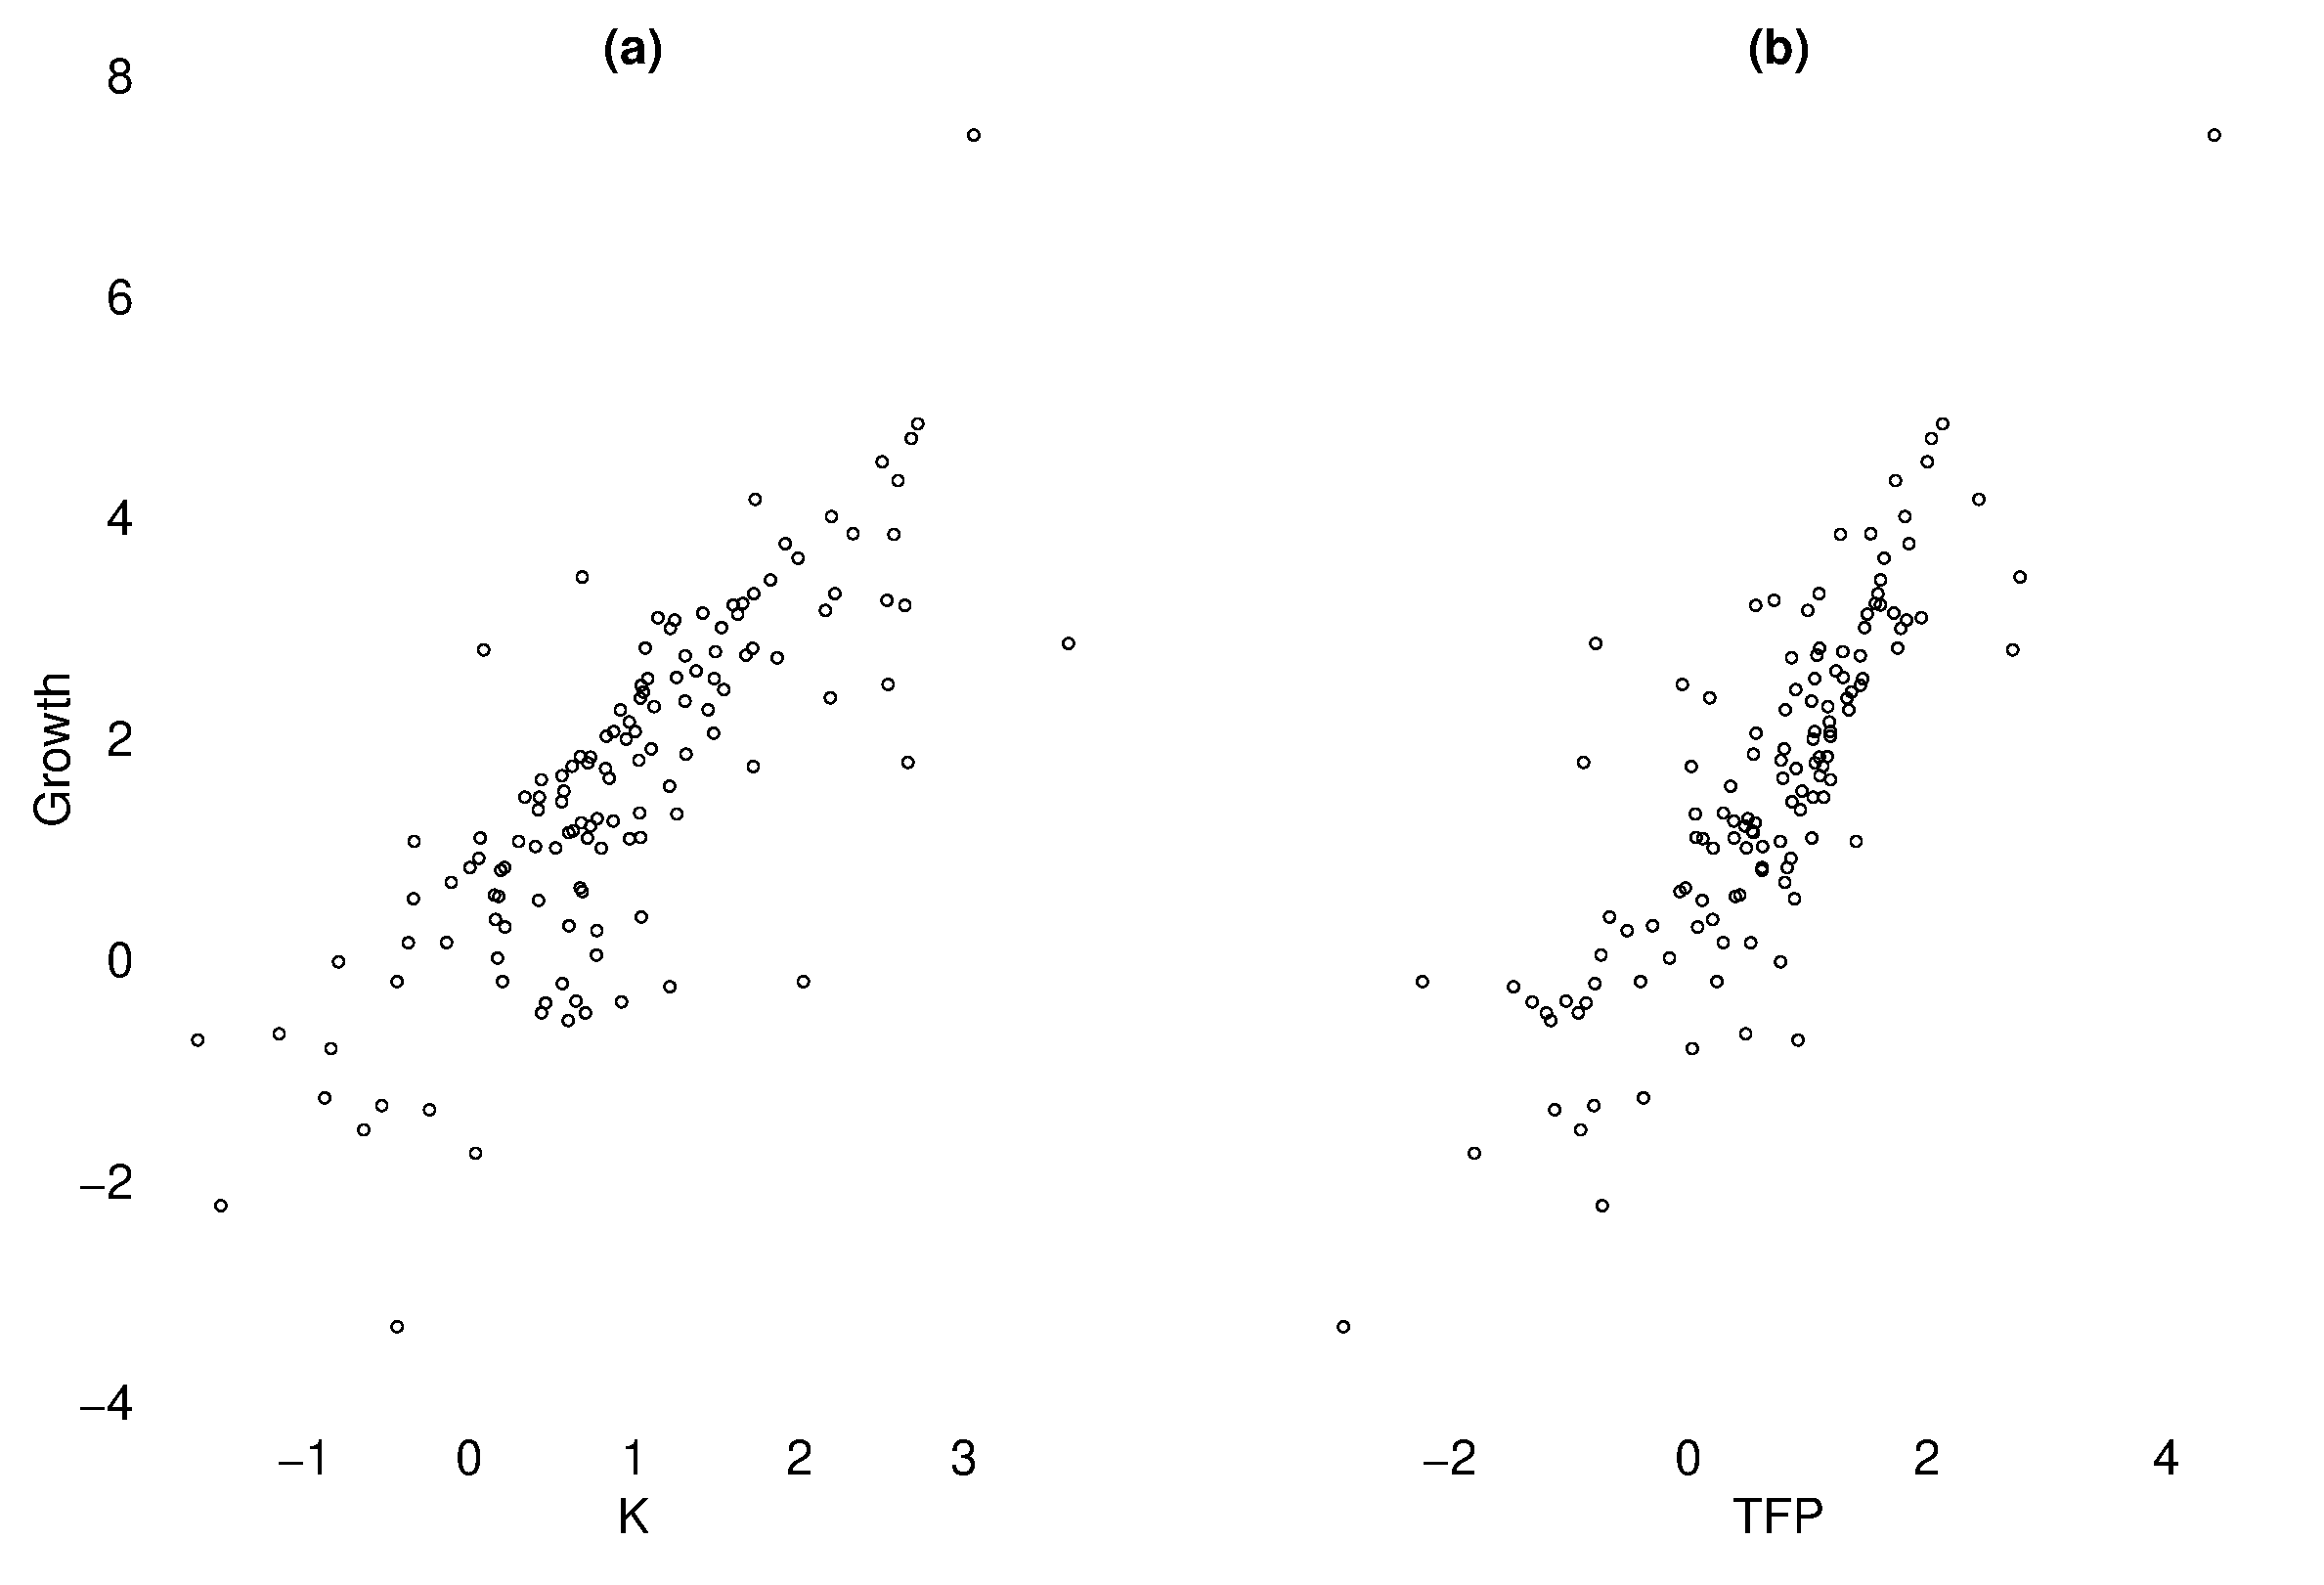
\includegraphics[scale=.3]{growth.eps}
  \end{figure}
\end{frame}
%--------------------------------------

%--------------------------------------
\begin{frame}
  \begin{figure}
    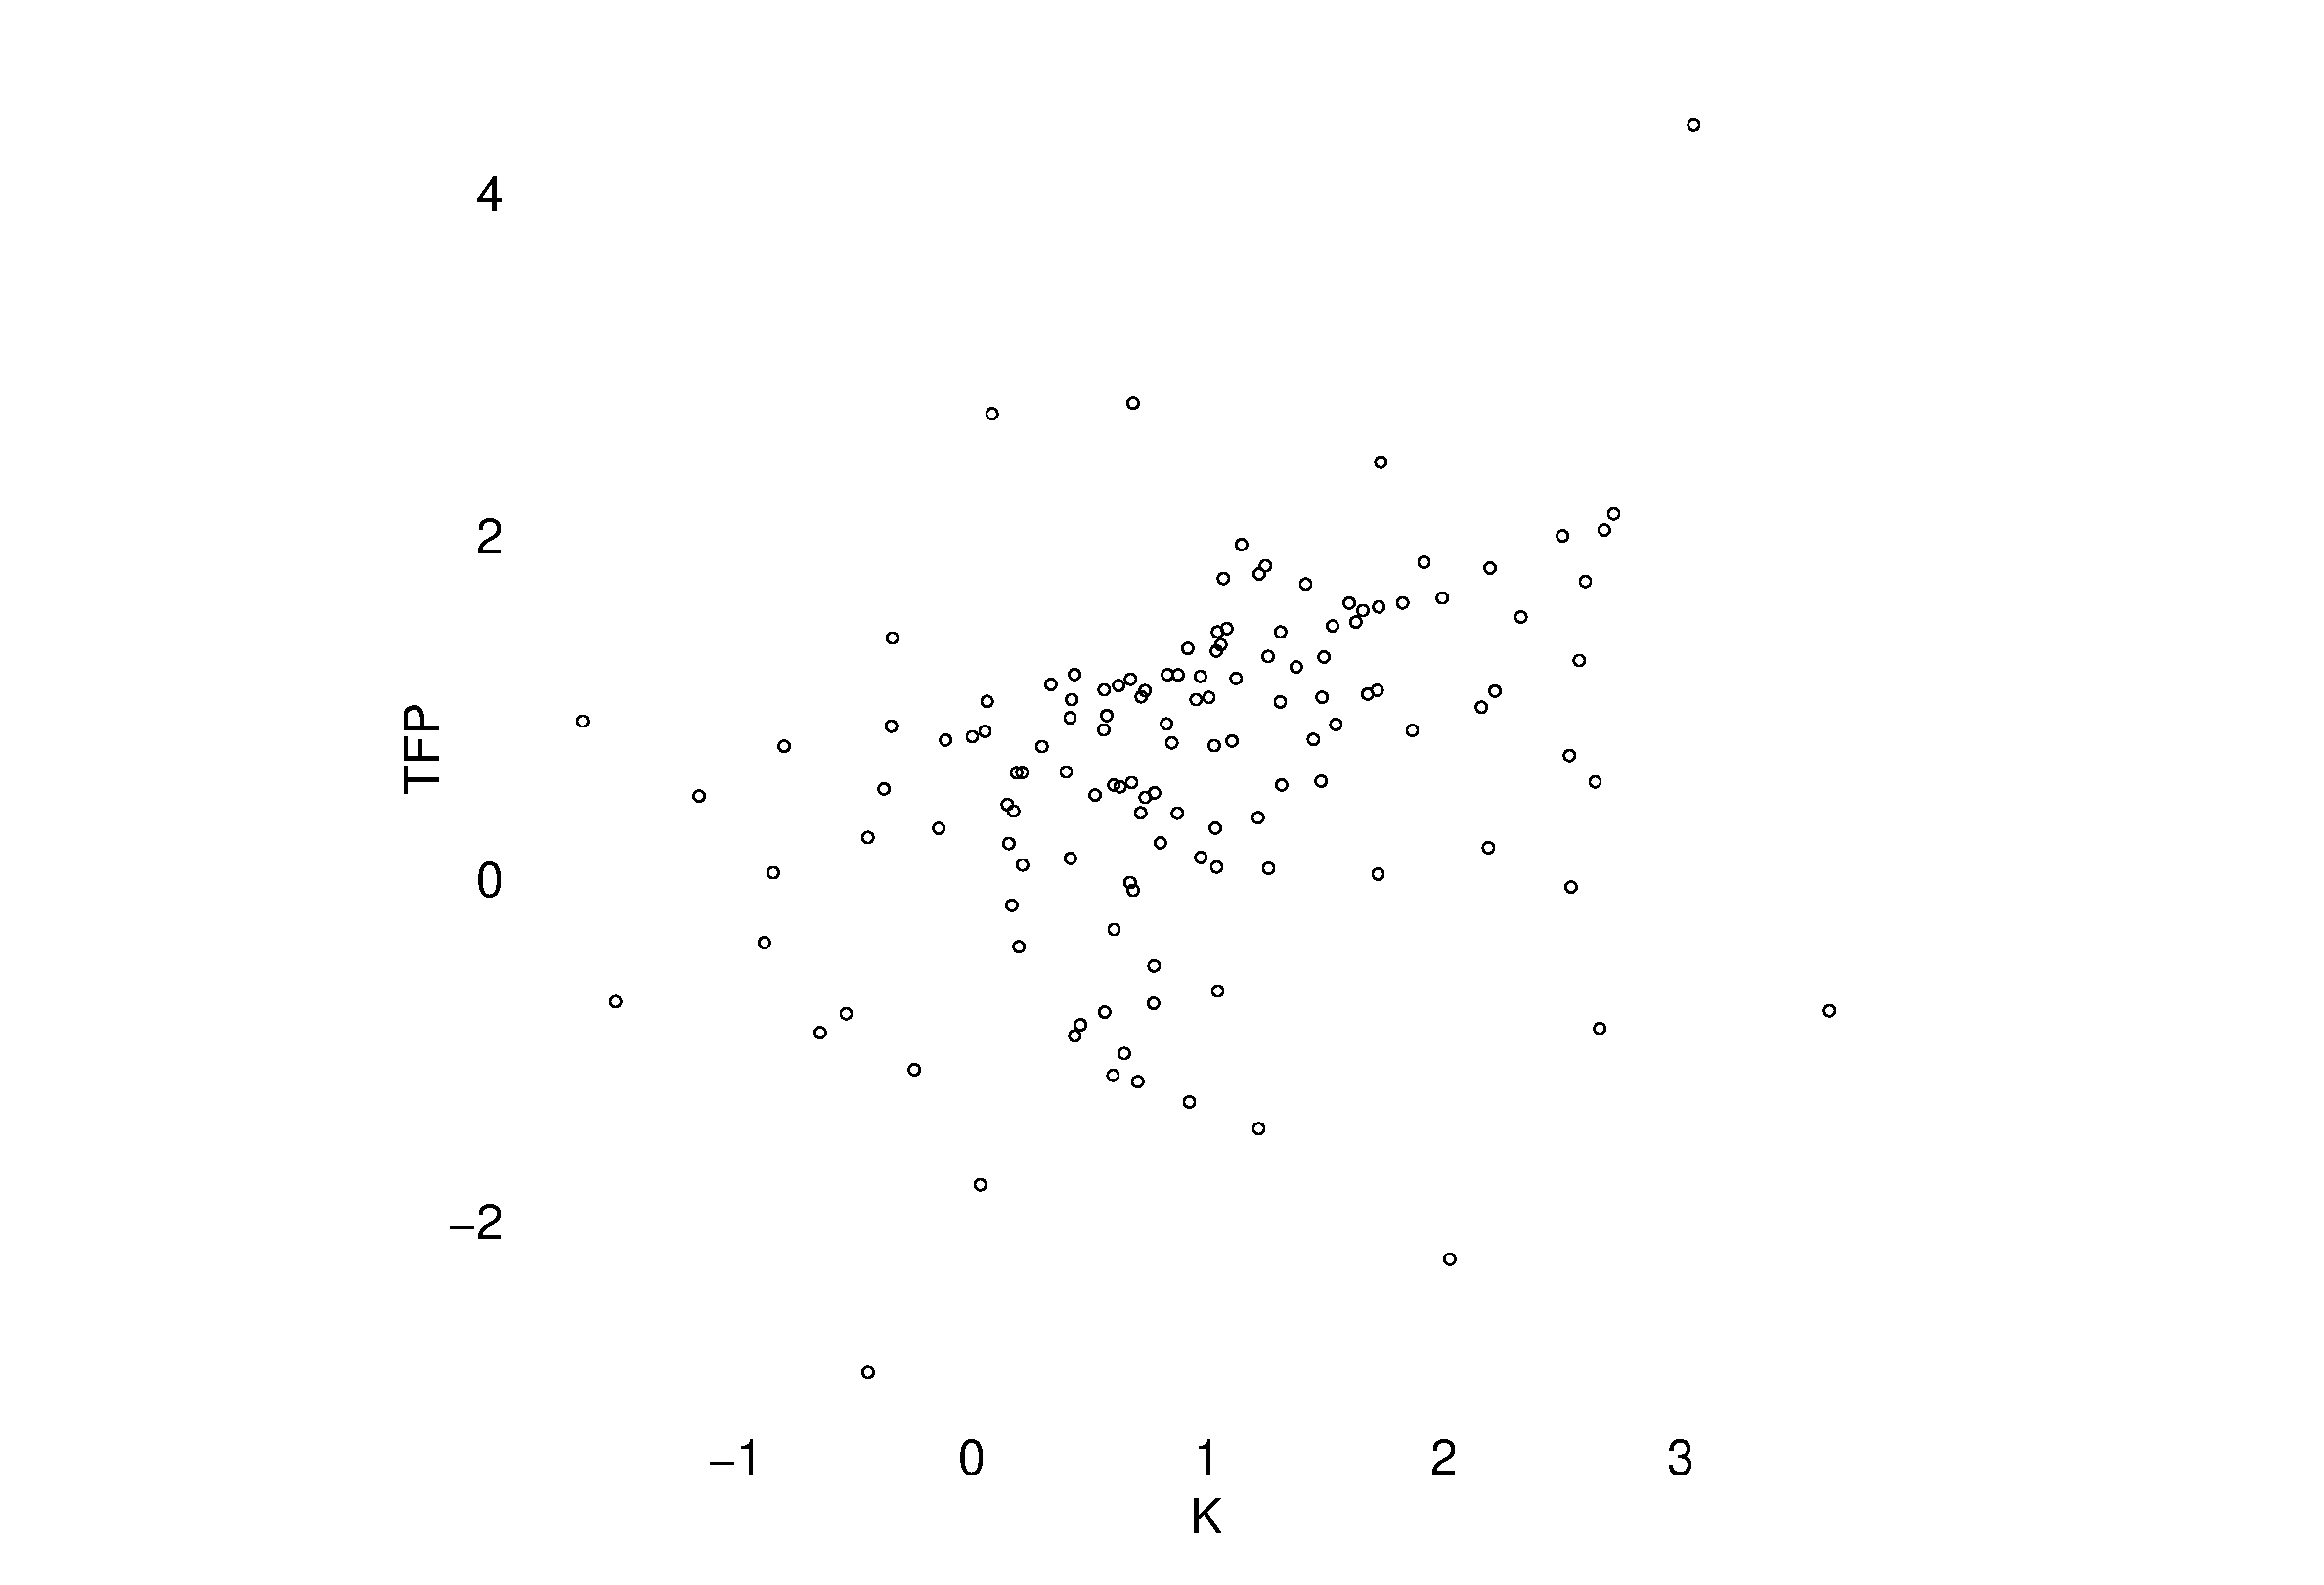
\includegraphics[scale=.3]{growth2.eps}
  \end{figure}
\end{frame}
%--------------------------------------

%--------------------------------------
\begin{frame}
One important factor with regard to the reduction in productivity growth is the slow growth rate of the labour force. 
In recent years the US labour force has flattened out after years of increasing number of people available for work due to
\begin{enumerate}
  \item Population growth
  \item Female labour participation
  \item Immigration
\end{enumerate}
\medskip
An important long-term demographic trend, that also affects other developed countries is the ageing of the baby boom generation. 
As more and more people from this generation start to retire, the dependency ratio starts to increase significantly.
The dependency ratio is the ratio of non-working to working people.  
\end{frame}
%--------------------------------------

%--------------------------------------
\begin{frame}
  \begin{figure}
    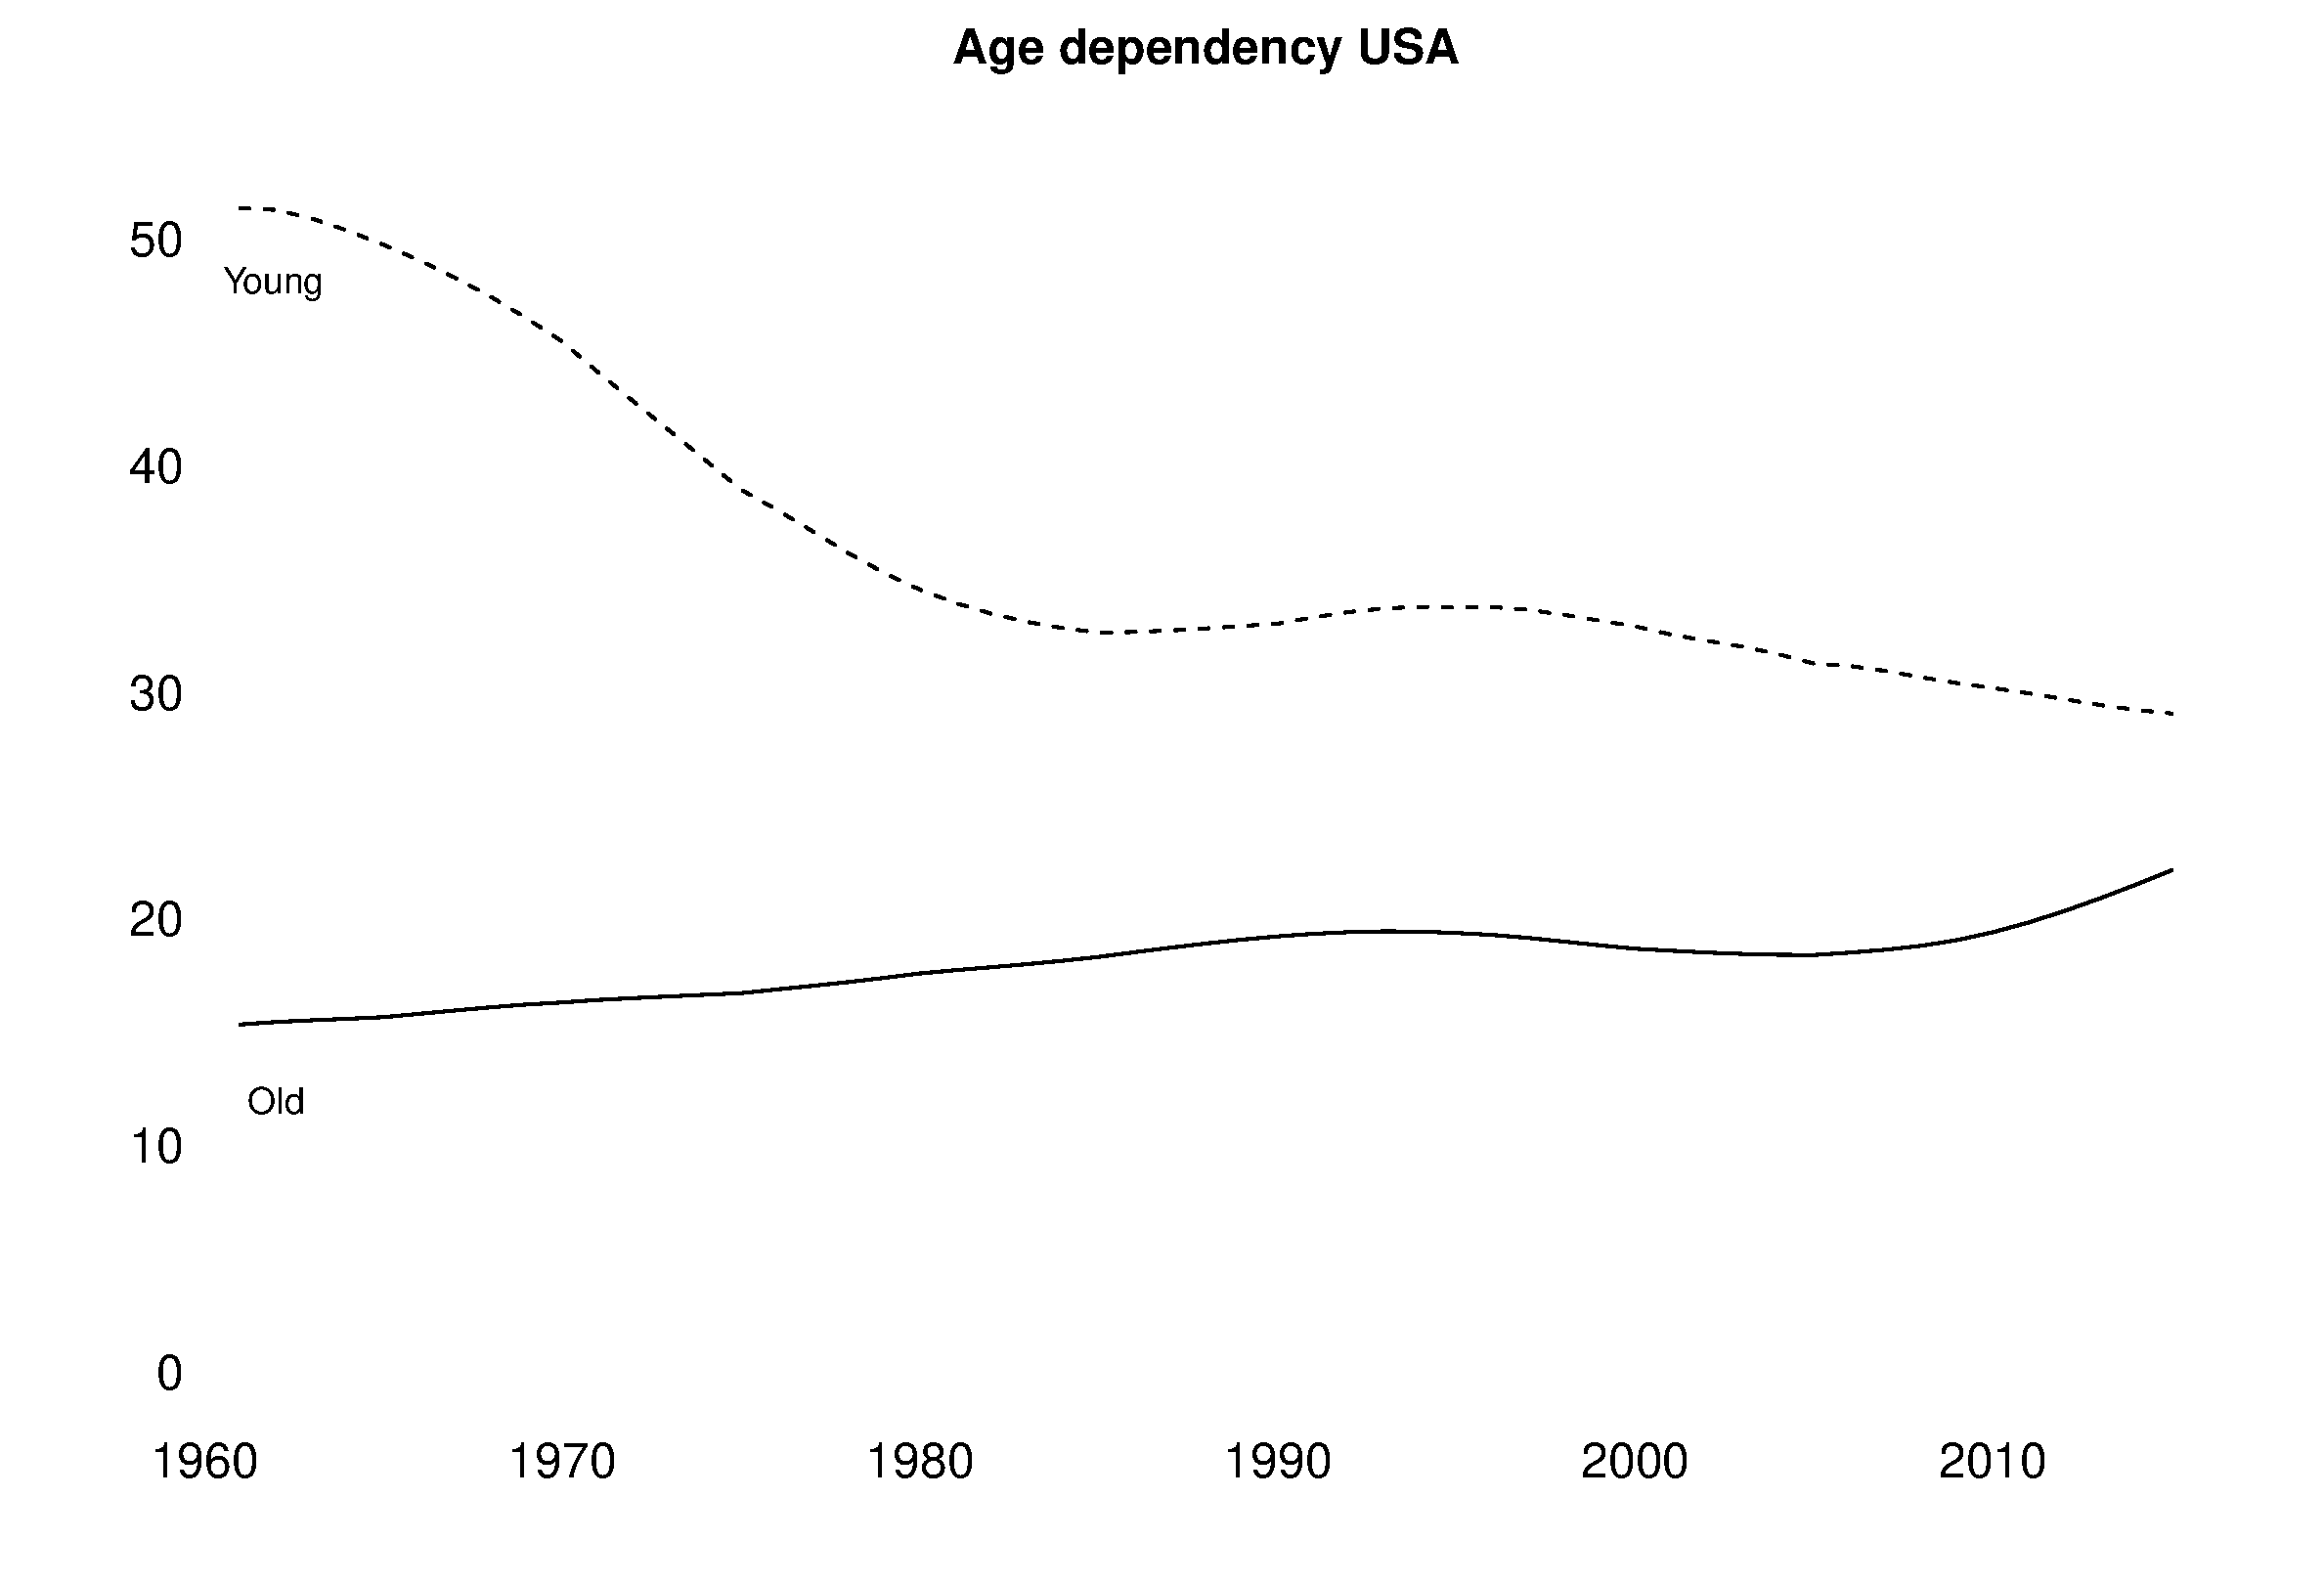
\includegraphics[scale=.3]{age_usa.eps}
  \end{figure}
\end{frame}
%--------------------------------------

%--------------------------------------
\begin{frame}
  \begin{figure}
    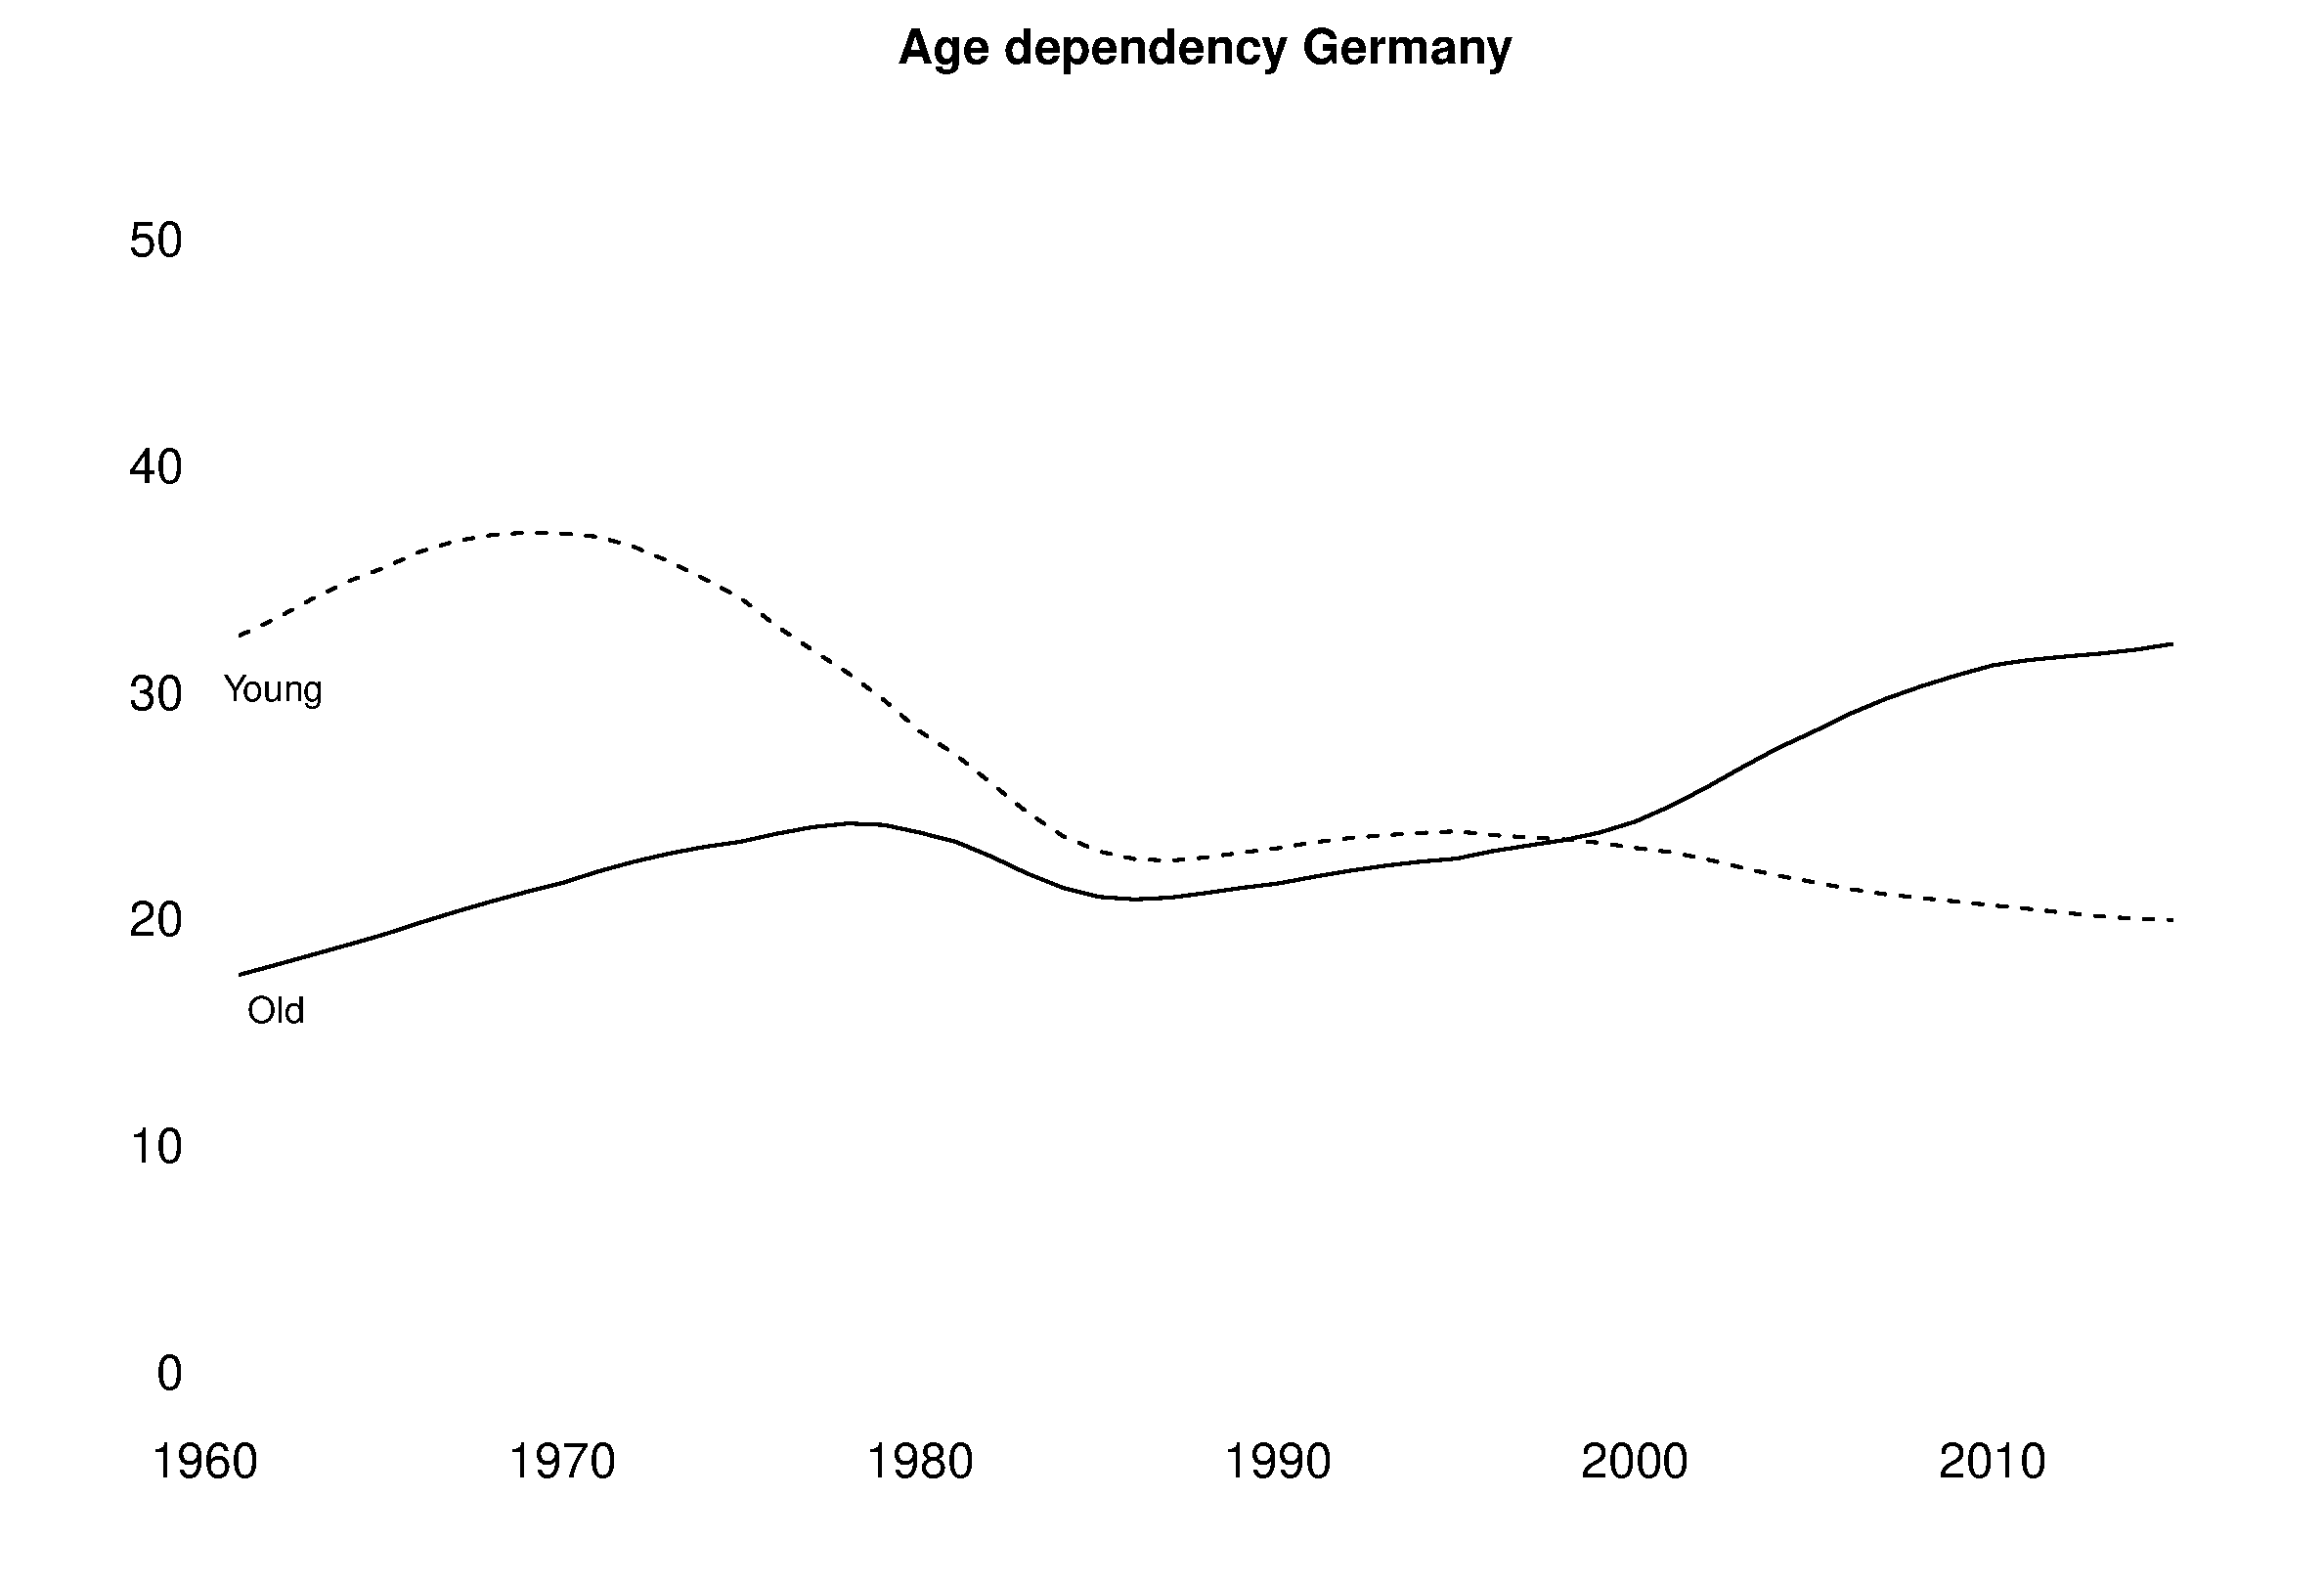
\includegraphics[scale=.3]{age_ger.eps}
  \end{figure}
\end{frame}
%--------------------------------------

%--------------------------------------
\begin{frame}
  \begin{figure}
    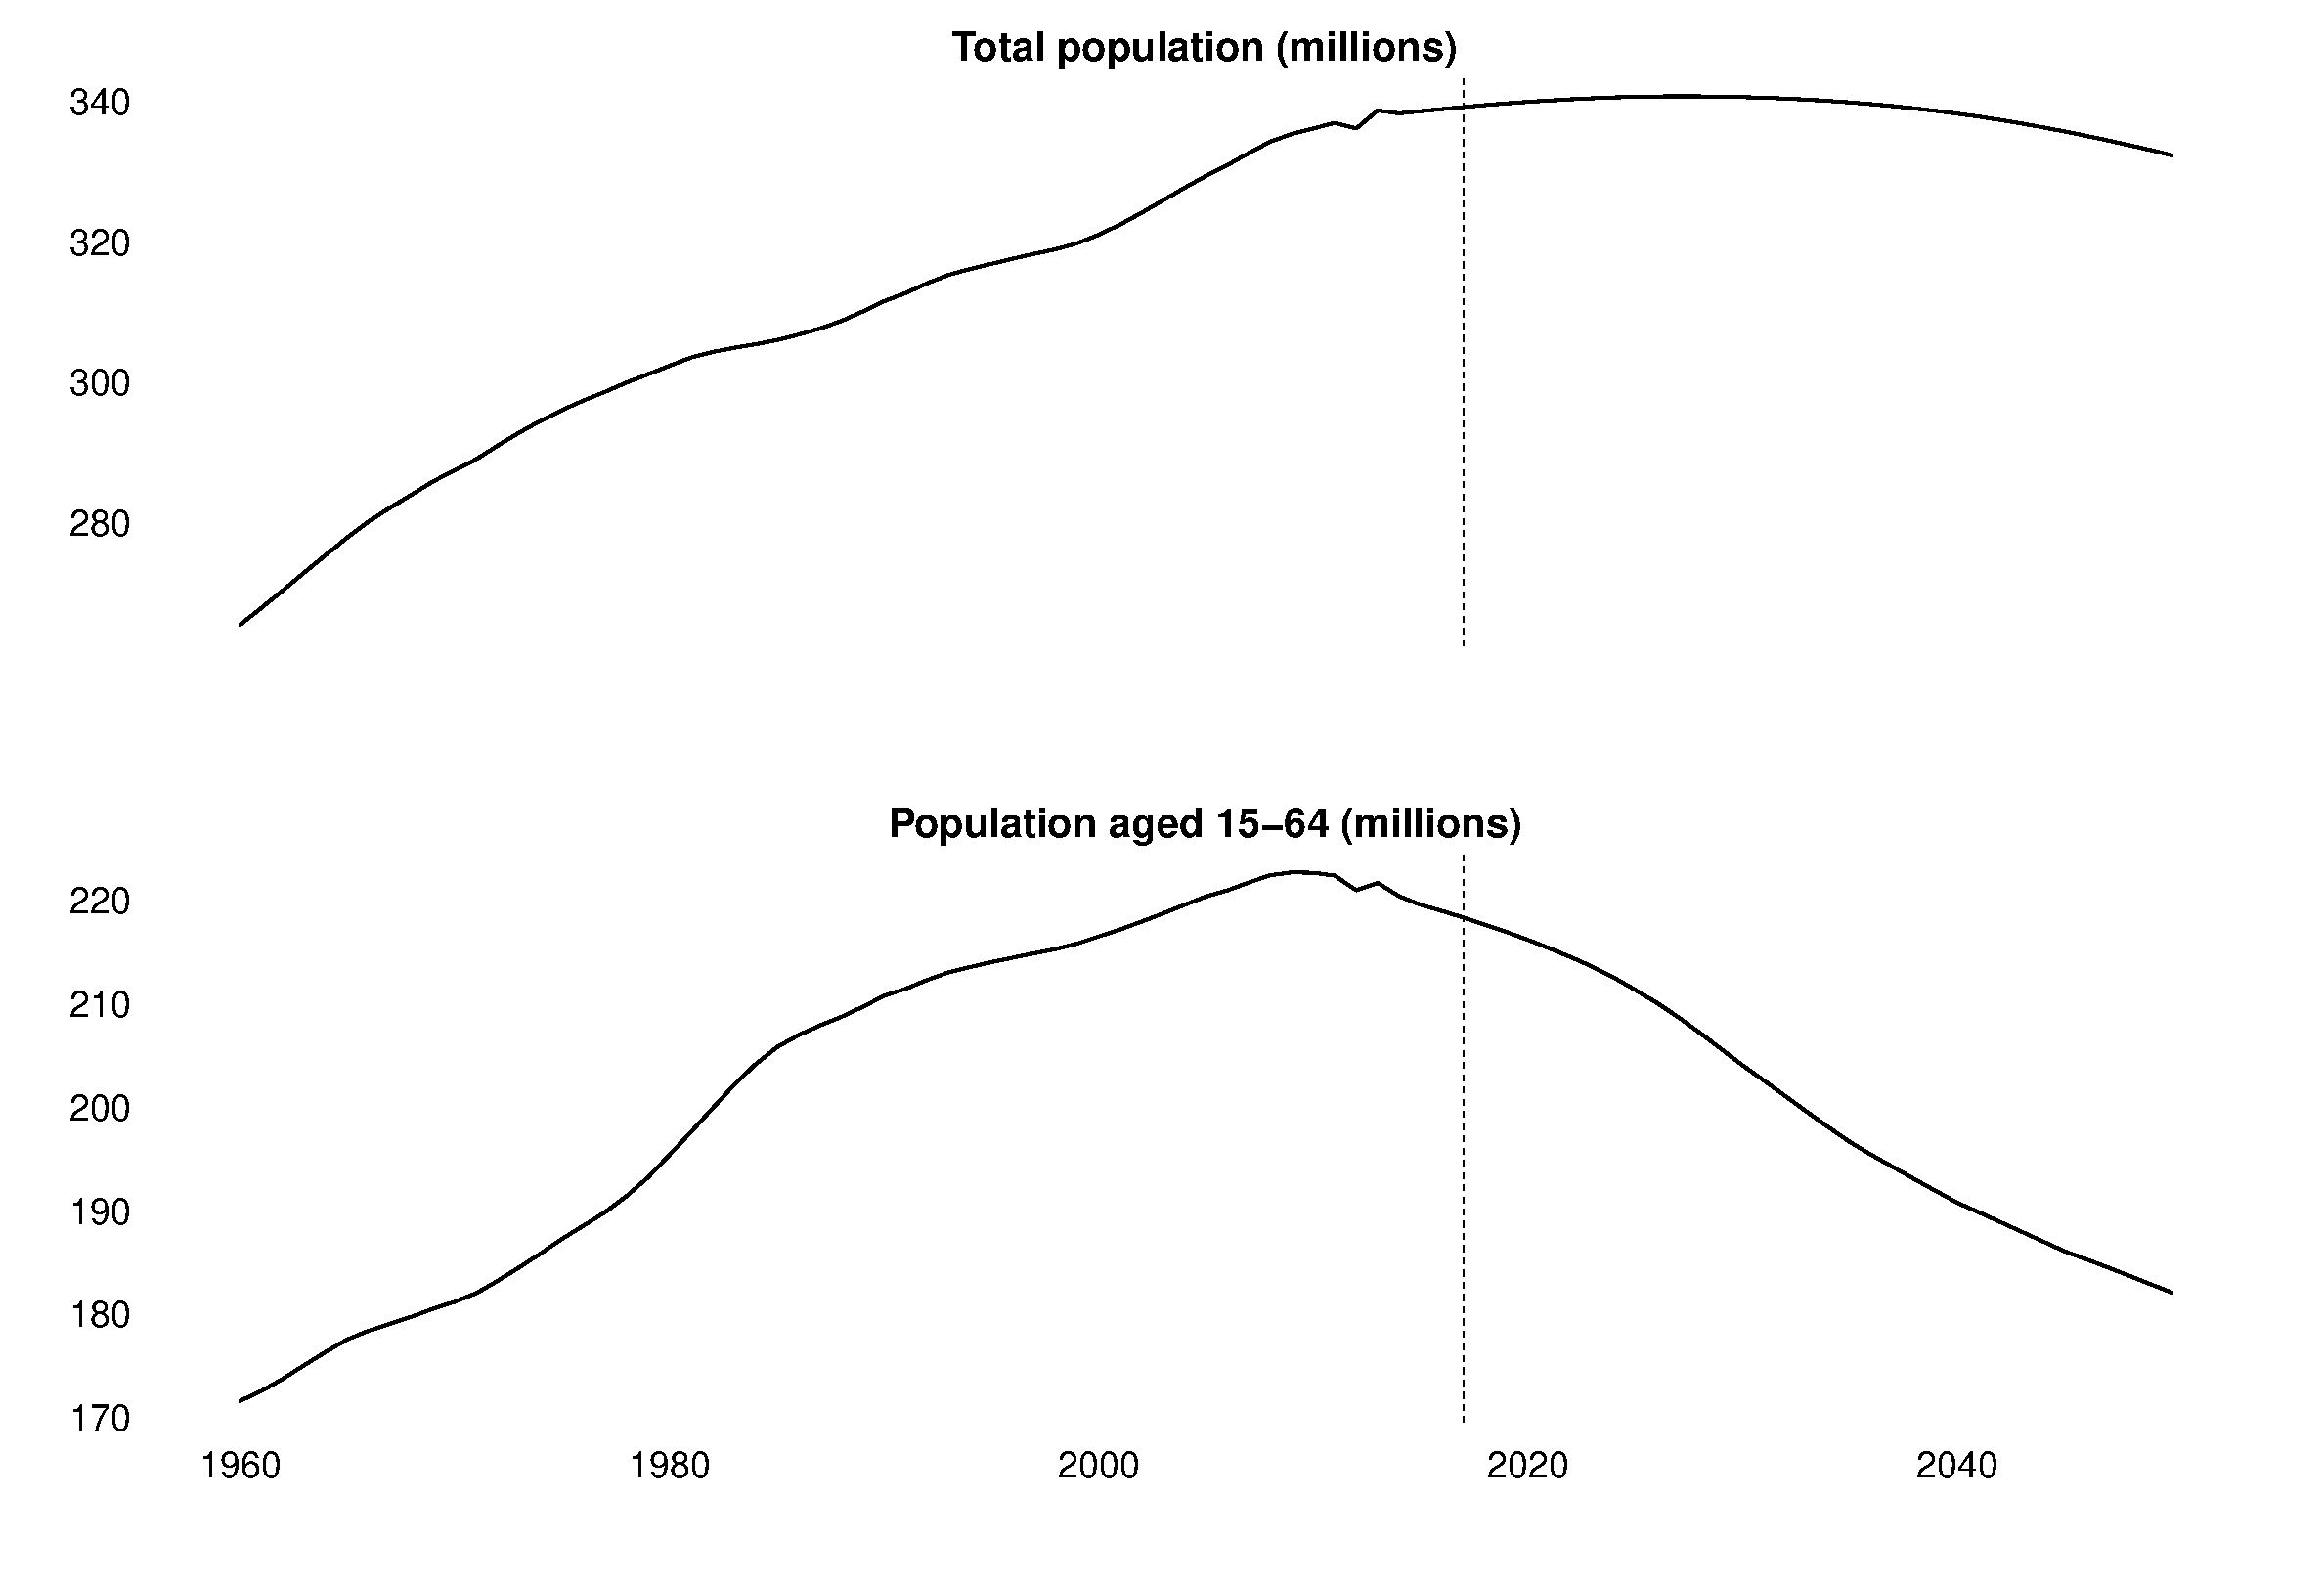
\includegraphics[scale=.3]{population_projection.eps}
  \end{figure}
\end{frame}
%--------------------------------------

%--------------------------------------
\begin{frame}
  One serious challenge for future economic growth in Europe is dealing with the demographic changes, specifically the effects of an ageing population.
Population growth is slowing and to peak in the middle of the century.
Worryingly, the working population, those aged between 15-64 years, has peaked already and is set to decline. 
The macroeconomic problems that Europe faces are twofold
\begin{itemize}
  \item Short term
  \begin{itemize}
    \item Weak aggregate demand
    \item High levels of public and private debt
  \end{itemize}
  \item Long term
  \begin{itemize}
    \item Demographic challenges
    \item Requiring productivity increase, immigration, higher ages for retirement
  \end{itemize}
\end{itemize}
\end{frame}
%--------------------------------------

%--------------------------------------
\begin{frame}
 Young (1992) provides a growth accounting study focusing on Hong Kong and Singapore
 \begin{itemize}
   \item Both cities have been very successful in restructuring their economy; Hong Kong experienced an economic growth of 147\% between the early 1970s and 1990, and Singapore 154\%
 \end{itemize}
 \medskip
 Young focuses on these two cities as they have a similar background yet are different on a number of issues emphasised by growth theory. 
  Some similarities in the prewar period include
  \begin{itemize}
    \item Both British colonies
    \item Entrep\^{o}t trading ports
  \item Little domestic manufacturing
  \end{itemize}
\end{frame}
%--------------------------------------

%--------------------------------------
\begin{frame}
  During the postwar period, both city-states developed export-dependent manufacturing industries, going from producing textiles to clothing, plastics, electronics, and since the 1980s shifting to banking and financial services.
  Two important differences between the cities are
\begin{enumerate}
  \item Hong Kong had a better educated population in the early postwar years
  \item Hong Kong has pursuit laissez faire policies, whereas Singapore implemented forced national savings and attracted a lot of foreign direct investment
\end{enumerate}
\end{frame}
%--------------------------------------

%--------------------------------------
\begin{frame}
  \begin{figure}
    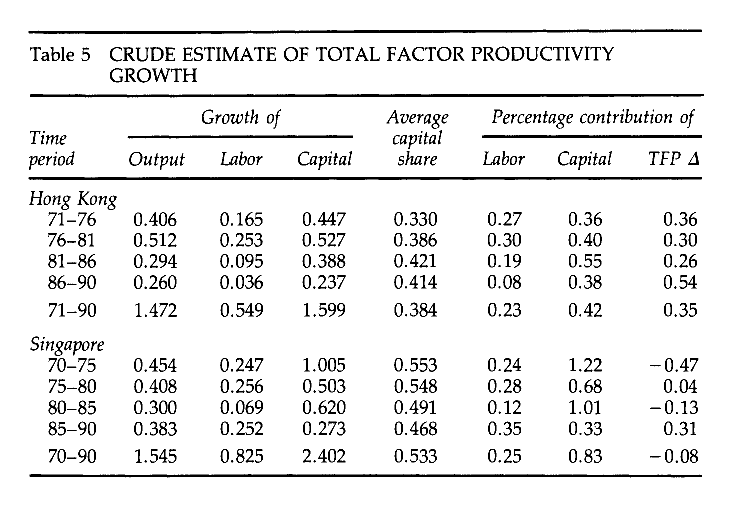
\includegraphics[scale=.8]{young.eps}
  \end{figure}
\end{frame}
%--------------------------------------

%--------------------------------------
\begin{frame}
  \begin{figure}
    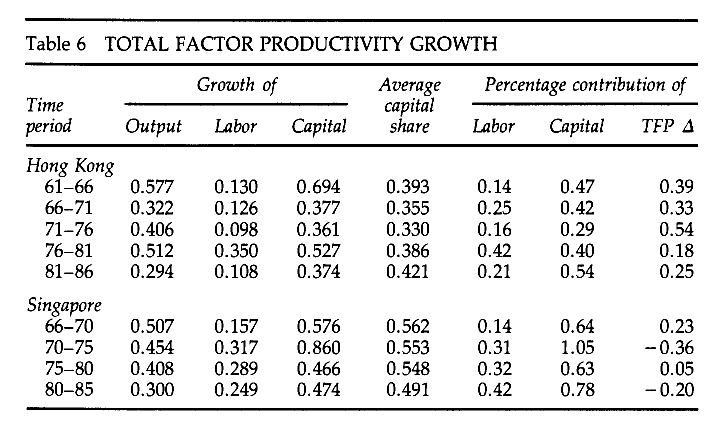
\includegraphics[scale=.8]{young2.eps}
  \end{figure}
\end{frame}
%--------------------------------------

%--------------------------------------
\begin{frame}
  Young finds that both cities experienced an economic transformation going roughly through the same industries
  \begin{itemize}
    \item Singapore seemed to have done this in a more compressed period
    \item Rate of structural transformation is 0.209 for Singapore, 0.082 for Hong Kong
    \item Structural transformation is here measured by the allocation of labour in across two-digit ISIC manufacturing sectors
  \end{itemize}  
\end{frame}
%--------------------------------------

%--------------------------------------
\begin{frame}
Important is the source of growth: Capital deepening or TFP growth
  \begin{itemize}
    \item TFP growth played important role in Hong Kong, contributing about 30 to 50\% to output growth, with an average of 35\% between 1971-1990
    \item In Singapore capital was key, contributing to 83\% of output growth (did not contribute to TFP growth)
  \end{itemize}
  \medskip
  One advantage of TFP growth over growth based on capital accumulation is that it is more sustainable over the long run.   
\end{frame}
%--------------------------------------


%--------------------------------------
\begin{frame}
Young provides a theoretical explanation for the different patterns across the two cities focusing on
\begin{enumerate}
  \item Innovations ($N$)
  \item Bounded learning by doing ($T$)
\end{enumerate}
This is to account for the fact that new technologies do not achieve their full productivity potential directly upon implementation but that there are gains made by continuous adjustments.
\end{frame}
%--------------------------------------

%--------------------------------------
\begin{frame}
  \begin{figure}
    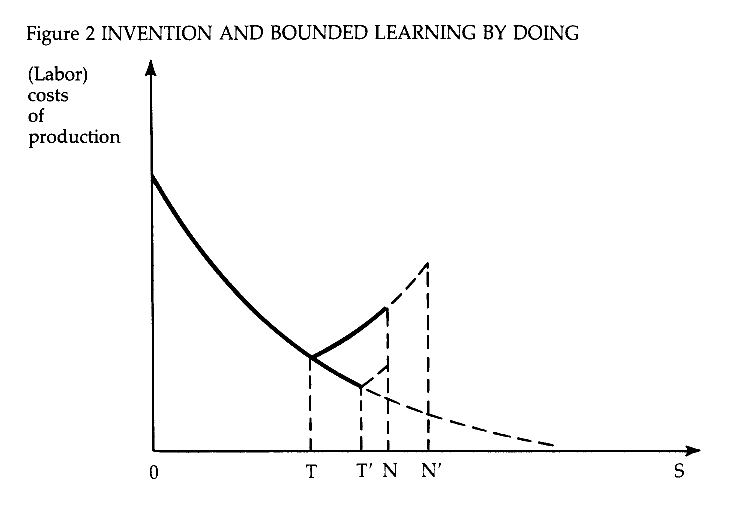
\includegraphics[scale=.8]{young3.eps}
  \end{figure}
\end{frame}
%--------------------------------------

%--------------------------------------
\begin{frame}
  \begin{figure}
    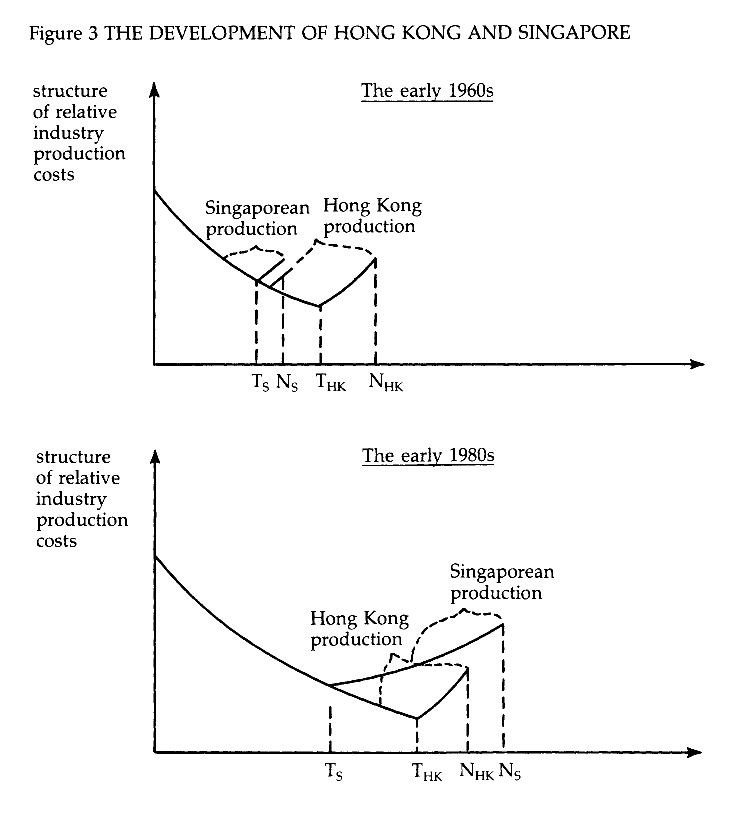
\includegraphics[scale=.7]{young4.eps}
  \end{figure}
\end{frame}
%--------------------------------------

%--------------------------------------
\begin{frame}
  Young argues that
\begin{itemize}
  \item In the early 1960s Hong Kong learning maturity was greater than that of Singapore: $T_{HK}>T_S$
  \item Hong Kong found it easier to copy technologies and enter new sectors: length of $[T_{HK},N_{HK}]$ relative to $[T_{S},N_{S}]$
  \item By the early 1980s Singapore had caught up, and both economies experienced substantial learning by doing: Rightward movement of $T_{HK},T_S$  
\end{itemize}
\end{frame}
%--------------------------------------

%--------------------------------------
\begin{frame}
  Cross-country evidence on grwoth determinants is often discounted
  \begin{itemize}
    \item Major issue is that there are many candidate models and choice in variable selection leaves room for data mining
  \end{itemize}
  \medskip
  Ciccone \& Jarocinski (2010) examine the sensitivity of results to changes in data and variable selection using Bayesian Model Averaging
  \begin{itemize}
    \item They find that the results are very sensitive to measurement error in income estimates
  \end{itemize}  
\end{frame}
%--------------------------------------

%--------------------------------------
\begin{frame}
  Consider a dataset with $N$ countries, where $N$ is relatively large to the number of possible variables $K$
  \begin{itemize}
    \item Could regress growth rate on all $K$ variables; likely find some statistically significant results
    \item If $N$ is close to $K$, the estimates will be imprecise (not feasible when $N>K$)
  \end{itemize}
  \medskip
  Bayesian methods aims to identify the determinants in terms of uncertainty about the true set of explanatory variables. 
\end{frame}
%--------------------------------------

%--------------------------------------
\begin{frame}
  All $K$ variables are collected in vector $x$; can denote the $2^K$ subsets of $x$ by $x_j$ and regress model
  \begin{align}
    y_n=\alpha +x_{jn}\beta_j + \epsilon_{jn}
  \end{align}
  $y_n$ is the growth rate of per capita GDP in country $n$. \\
  For the BMA all we further need is 
  \begin{enumerate}
    \item Priors for models $p_j$
    \item Priors for parameters $\alpha,\beta$ and variance of $\epsilon$
    \item Likelihood function for each model $j$
  \end{enumerate}
\end{frame}
%--------------------------------------

%--------------------------------------
\begin{frame}
  Important is the likelihood of model $j$ integrated with respect to the parameters using their prior distribution.
  The marginal likelihood of model $j$ can be written as
  \begin{align}
    l_y(M_j)
  \end{align}
  This is the density of the data conditional on the model, and in the Bayesian framework this can be translated into a posterior probability of the model conditional on the observed data
  \begin{align}
    p(M_j|y) \propto l_y(M_j)p_j
  \end{align}
  \medskip
  Finally, one can get the posterior inclusion probability for variable $k$ by summing the posterior probabilities of all models including the variable.
\end{frame}


%--------------------------------------
\begin{frame}
  \begin{figure}
    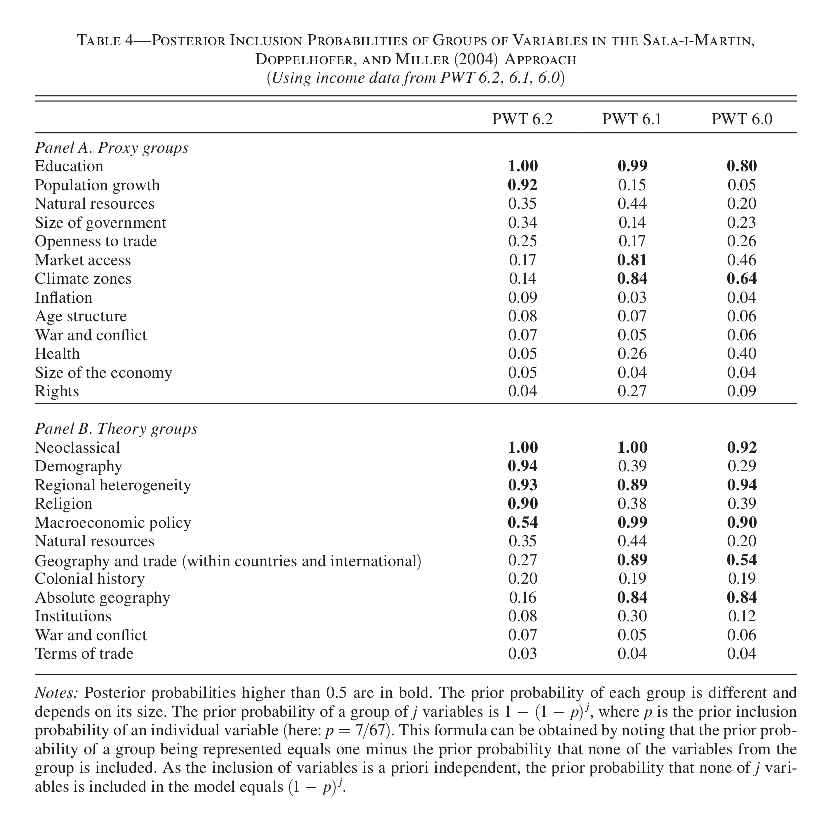
\includegraphics[scale=.5]{ciccone.eps}
  \end{figure}
\end{frame}
%--------------------------------------


%--------------------------------------
\end{document}
